\documentclass[11pt]{article}
\newcommand{\tablelang}{uk}
% Shared preamble for paper/manuscript/tex/{en,uk}/main.tex (XeLaTeX via Tectonic).
% Layout copied from the author's FFT preprint (Zenodo 23375871) so both papers share one house style.
% The including file sets \mainlang{english} or \mainlang{ukrainian} before % Shared preamble for paper/manuscript/tex/{en,uk}/main.tex (XeLaTeX via Tectonic).
% Layout copied from the author's FFT preprint (Zenodo 23375871) so both papers share one house style.
% The including file sets \mainlang{english} or \mainlang{ukrainian} before % Shared preamble for paper/manuscript/tex/{en,uk}/main.tex (XeLaTeX via Tectonic).
% Layout copied from the author's FFT preprint (Zenodo 23375871) so both papers share one house style.
% The including file sets \mainlang{english} or \mainlang{ukrainian} before \input{../preamble}.
\usepackage[a4paper,margin=25mm]{geometry}
\usepackage{fontspec}
\setmainfont{cmunrm.otf}[BoldFont=cmunbx.otf,ItalicFont=cmunti.otf,BoldItalicFont=cmunbi.otf]
\setsansfont{cmunss.otf}[BoldFont=cmunsx.otf,ItalicFont=cmunsi.otf]
\setmonofont{cmuntt.otf}[BoldFont=cmuntb.otf,ItalicFont=cmunit.otf]
\usepackage[ukrainian,english]{babel}
\usepackage{amsmath,amssymb,amsthm,mathtools}
\usepackage{booktabs,tabularx,array,multirow}
\usepackage{graphicx}
\usepackage[font=small,labelfont=bf]{caption}
\usepackage{subcaption}
\usepackage{xcolor}
\usepackage{enumitem}
\usepackage{microtype}
\usepackage[numbers,sort&compress]{natbib}
\PassOptionsToPackage{hyphens}{url}
\usepackage[hidelinks]{hyperref}
\usepackage[nameinlink,capitalise,noabbrev]{cleveref}
\usepackage{url}
\usepackage{etoolbox}
\AtBeginEnvironment{thebibliography}{\raggedright}

\graphicspath{{../../figures/}{../../generated/figures/}}
% primitive input: LaTeX's \input is not expandable and breaks inside tabular after \midrule
\makeatletter\newcommand{\gentable}[1]{\@@input ../tables/\tablelang/T#1.tex }\makeatother

% notation (archive-index paper)
\newcommand{\code}[1]{\texttt{#1}}
\newcommand{\sys}[1]{\textsf{#1}}          % system names in tables and text: \sys{adaptive}
\newcommand{\metric}[1]{\mathrm{#1}}       % nDCG@10 etc. in math
\newcommand{\uapar}{UA-PAR}
% \pending{...}: text not written yet. Visible in the PDF; paper/release/compliance.py rejects any PDF that has one.
\newcommand{\pending}[1]{\textcolor{red}{[PENDING: #1]}}

% theorem names: the including file may define these before \input{../preamble}
\providecommand{\lemmaname}{Lemma}
\providecommand{\propositionname}{Proposition}
\providecommand{\definitionname}{Definition}
\providecommand{\remarkname}{Remark}
\providecommand{\corollaryname}{Corollary}
\providecommand{\theoremname}{Theorem}
\theoremstyle{plain}
\newtheorem{lemma}{\lemmaname}
\newtheorem{proposition}{\propositionname}
\theoremstyle{definition}
\newtheorem{definition}{\definitionname}
\theoremstyle{remark}
\newtheorem{remark}{\remarkname}

\setlength{\tabcolsep}{4pt}
\renewcommand{\arraystretch}{1.12}
\sloppy
.
\usepackage[a4paper,margin=25mm]{geometry}
\usepackage{fontspec}
\setmainfont{cmunrm.otf}[BoldFont=cmunbx.otf,ItalicFont=cmunti.otf,BoldItalicFont=cmunbi.otf]
\setsansfont{cmunss.otf}[BoldFont=cmunsx.otf,ItalicFont=cmunsi.otf]
\setmonofont{cmuntt.otf}[BoldFont=cmuntb.otf,ItalicFont=cmunit.otf]
\usepackage[ukrainian,english]{babel}
\usepackage{amsmath,amssymb,amsthm,mathtools}
\usepackage{booktabs,tabularx,array,multirow}
\usepackage{graphicx}
\usepackage[font=small,labelfont=bf]{caption}
\usepackage{subcaption}
\usepackage{xcolor}
\usepackage{enumitem}
\usepackage{microtype}
\usepackage[numbers,sort&compress]{natbib}
\PassOptionsToPackage{hyphens}{url}
\usepackage[hidelinks]{hyperref}
\usepackage[nameinlink,capitalise,noabbrev]{cleveref}
\usepackage{url}
\usepackage{etoolbox}
\AtBeginEnvironment{thebibliography}{\raggedright}

\graphicspath{{../../figures/}{../../generated/figures/}}
% primitive input: LaTeX's \input is not expandable and breaks inside tabular after \midrule
\makeatletter\newcommand{\gentable}[1]{\@@input ../tables/\tablelang/T#1.tex }\makeatother

% notation (archive-index paper)
\newcommand{\code}[1]{\texttt{#1}}
\newcommand{\sys}[1]{\textsf{#1}}          % system names in tables and text: \sys{adaptive}
\newcommand{\metric}[1]{\mathrm{#1}}       % nDCG@10 etc. in math
\newcommand{\uapar}{UA-PAR}
% \pending{...}: text not written yet. Visible in the PDF; paper/release/compliance.py rejects any PDF that has one.
\newcommand{\pending}[1]{\textcolor{red}{[PENDING: #1]}}

% theorem names: the including file may define these before % Shared preamble for paper/manuscript/tex/{en,uk}/main.tex (XeLaTeX via Tectonic).
% Layout copied from the author's FFT preprint (Zenodo 23375871) so both papers share one house style.
% The including file sets \mainlang{english} or \mainlang{ukrainian} before \input{../preamble}.
\usepackage[a4paper,margin=25mm]{geometry}
\usepackage{fontspec}
\setmainfont{cmunrm.otf}[BoldFont=cmunbx.otf,ItalicFont=cmunti.otf,BoldItalicFont=cmunbi.otf]
\setsansfont{cmunss.otf}[BoldFont=cmunsx.otf,ItalicFont=cmunsi.otf]
\setmonofont{cmuntt.otf}[BoldFont=cmuntb.otf,ItalicFont=cmunit.otf]
\usepackage[ukrainian,english]{babel}
\usepackage{amsmath,amssymb,amsthm,mathtools}
\usepackage{booktabs,tabularx,array,multirow}
\usepackage{graphicx}
\usepackage[font=small,labelfont=bf]{caption}
\usepackage{subcaption}
\usepackage{xcolor}
\usepackage{enumitem}
\usepackage{microtype}
\usepackage[numbers,sort&compress]{natbib}
\PassOptionsToPackage{hyphens}{url}
\usepackage[hidelinks]{hyperref}
\usepackage[nameinlink,capitalise,noabbrev]{cleveref}
\usepackage{url}
\usepackage{etoolbox}
\AtBeginEnvironment{thebibliography}{\raggedright}

\graphicspath{{../../figures/}{../../generated/figures/}}
% primitive input: LaTeX's \input is not expandable and breaks inside tabular after \midrule
\makeatletter\newcommand{\gentable}[1]{\@@input ../tables/\tablelang/T#1.tex }\makeatother

% notation (archive-index paper)
\newcommand{\code}[1]{\texttt{#1}}
\newcommand{\sys}[1]{\textsf{#1}}          % system names in tables and text: \sys{adaptive}
\newcommand{\metric}[1]{\mathrm{#1}}       % nDCG@10 etc. in math
\newcommand{\uapar}{UA-PAR}
% \pending{...}: text not written yet. Visible in the PDF; paper/release/compliance.py rejects any PDF that has one.
\newcommand{\pending}[1]{\textcolor{red}{[PENDING: #1]}}

% theorem names: the including file may define these before \input{../preamble}
\providecommand{\lemmaname}{Lemma}
\providecommand{\propositionname}{Proposition}
\providecommand{\definitionname}{Definition}
\providecommand{\remarkname}{Remark}
\providecommand{\corollaryname}{Corollary}
\providecommand{\theoremname}{Theorem}
\theoremstyle{plain}
\newtheorem{lemma}{\lemmaname}
\newtheorem{proposition}{\propositionname}
\theoremstyle{definition}
\newtheorem{definition}{\definitionname}
\theoremstyle{remark}
\newtheorem{remark}{\remarkname}

\setlength{\tabcolsep}{4pt}
\renewcommand{\arraystretch}{1.12}
\sloppy

\providecommand{\lemmaname}{Lemma}
\providecommand{\propositionname}{Proposition}
\providecommand{\definitionname}{Definition}
\providecommand{\remarkname}{Remark}
\providecommand{\corollaryname}{Corollary}
\providecommand{\theoremname}{Theorem}
\theoremstyle{plain}
\newtheorem{lemma}{\lemmaname}
\newtheorem{proposition}{\propositionname}
\theoremstyle{definition}
\newtheorem{definition}{\definitionname}
\theoremstyle{remark}
\newtheorem{remark}{\remarkname}

\setlength{\tabcolsep}{4pt}
\renewcommand{\arraystretch}{1.12}
\sloppy
.
\usepackage[a4paper,margin=25mm]{geometry}
\usepackage{fontspec}
\setmainfont{cmunrm.otf}[BoldFont=cmunbx.otf,ItalicFont=cmunti.otf,BoldItalicFont=cmunbi.otf]
\setsansfont{cmunss.otf}[BoldFont=cmunsx.otf,ItalicFont=cmunsi.otf]
\setmonofont{cmuntt.otf}[BoldFont=cmuntb.otf,ItalicFont=cmunit.otf]
\usepackage[ukrainian,english]{babel}
\usepackage{amsmath,amssymb,amsthm,mathtools}
\usepackage{booktabs,tabularx,array,multirow}
\usepackage{graphicx}
\usepackage[font=small,labelfont=bf]{caption}
\usepackage{subcaption}
\usepackage{xcolor}
\usepackage{enumitem}
\usepackage{microtype}
\usepackage[numbers,sort&compress]{natbib}
\PassOptionsToPackage{hyphens}{url}
\usepackage[hidelinks]{hyperref}
\usepackage[nameinlink,capitalise,noabbrev]{cleveref}
\usepackage{url}
\usepackage{etoolbox}
\AtBeginEnvironment{thebibliography}{\raggedright}

\graphicspath{{../../figures/}{../../generated/figures/}}
% primitive input: LaTeX's \input is not expandable and breaks inside tabular after \midrule
\makeatletter\newcommand{\gentable}[1]{\@@input ../tables/\tablelang/T#1.tex }\makeatother

% notation (archive-index paper)
\newcommand{\code}[1]{\texttt{#1}}
\newcommand{\sys}[1]{\textsf{#1}}          % system names in tables and text: \sys{adaptive}
\newcommand{\metric}[1]{\mathrm{#1}}       % nDCG@10 etc. in math
\newcommand{\uapar}{UA-PAR}
% \pending{...}: text not written yet. Visible in the PDF; paper/release/compliance.py rejects any PDF that has one.
\newcommand{\pending}[1]{\textcolor{red}{[PENDING: #1]}}

% theorem names: the including file may define these before % Shared preamble for paper/manuscript/tex/{en,uk}/main.tex (XeLaTeX via Tectonic).
% Layout copied from the author's FFT preprint (Zenodo 23375871) so both papers share one house style.
% The including file sets \mainlang{english} or \mainlang{ukrainian} before % Shared preamble for paper/manuscript/tex/{en,uk}/main.tex (XeLaTeX via Tectonic).
% Layout copied from the author's FFT preprint (Zenodo 23375871) so both papers share one house style.
% The including file sets \mainlang{english} or \mainlang{ukrainian} before \input{../preamble}.
\usepackage[a4paper,margin=25mm]{geometry}
\usepackage{fontspec}
\setmainfont{cmunrm.otf}[BoldFont=cmunbx.otf,ItalicFont=cmunti.otf,BoldItalicFont=cmunbi.otf]
\setsansfont{cmunss.otf}[BoldFont=cmunsx.otf,ItalicFont=cmunsi.otf]
\setmonofont{cmuntt.otf}[BoldFont=cmuntb.otf,ItalicFont=cmunit.otf]
\usepackage[ukrainian,english]{babel}
\usepackage{amsmath,amssymb,amsthm,mathtools}
\usepackage{booktabs,tabularx,array,multirow}
\usepackage{graphicx}
\usepackage[font=small,labelfont=bf]{caption}
\usepackage{subcaption}
\usepackage{xcolor}
\usepackage{enumitem}
\usepackage{microtype}
\usepackage[numbers,sort&compress]{natbib}
\PassOptionsToPackage{hyphens}{url}
\usepackage[hidelinks]{hyperref}
\usepackage[nameinlink,capitalise,noabbrev]{cleveref}
\usepackage{url}
\usepackage{etoolbox}
\AtBeginEnvironment{thebibliography}{\raggedright}

\graphicspath{{../../figures/}{../../generated/figures/}}
% primitive input: LaTeX's \input is not expandable and breaks inside tabular after \midrule
\makeatletter\newcommand{\gentable}[1]{\@@input ../tables/\tablelang/T#1.tex }\makeatother

% notation (archive-index paper)
\newcommand{\code}[1]{\texttt{#1}}
\newcommand{\sys}[1]{\textsf{#1}}          % system names in tables and text: \sys{adaptive}
\newcommand{\metric}[1]{\mathrm{#1}}       % nDCG@10 etc. in math
\newcommand{\uapar}{UA-PAR}
% \pending{...}: text not written yet. Visible in the PDF; paper/release/compliance.py rejects any PDF that has one.
\newcommand{\pending}[1]{\textcolor{red}{[PENDING: #1]}}

% theorem names: the including file may define these before \input{../preamble}
\providecommand{\lemmaname}{Lemma}
\providecommand{\propositionname}{Proposition}
\providecommand{\definitionname}{Definition}
\providecommand{\remarkname}{Remark}
\providecommand{\corollaryname}{Corollary}
\providecommand{\theoremname}{Theorem}
\theoremstyle{plain}
\newtheorem{lemma}{\lemmaname}
\newtheorem{proposition}{\propositionname}
\theoremstyle{definition}
\newtheorem{definition}{\definitionname}
\theoremstyle{remark}
\newtheorem{remark}{\remarkname}

\setlength{\tabcolsep}{4pt}
\renewcommand{\arraystretch}{1.12}
\sloppy
.
\usepackage[a4paper,margin=25mm]{geometry}
\usepackage{fontspec}
\setmainfont{cmunrm.otf}[BoldFont=cmunbx.otf,ItalicFont=cmunti.otf,BoldItalicFont=cmunbi.otf]
\setsansfont{cmunss.otf}[BoldFont=cmunsx.otf,ItalicFont=cmunsi.otf]
\setmonofont{cmuntt.otf}[BoldFont=cmuntb.otf,ItalicFont=cmunit.otf]
\usepackage[ukrainian,english]{babel}
\usepackage{amsmath,amssymb,amsthm,mathtools}
\usepackage{booktabs,tabularx,array,multirow}
\usepackage{graphicx}
\usepackage[font=small,labelfont=bf]{caption}
\usepackage{subcaption}
\usepackage{xcolor}
\usepackage{enumitem}
\usepackage{microtype}
\usepackage[numbers,sort&compress]{natbib}
\PassOptionsToPackage{hyphens}{url}
\usepackage[hidelinks]{hyperref}
\usepackage[nameinlink,capitalise,noabbrev]{cleveref}
\usepackage{url}
\usepackage{etoolbox}
\AtBeginEnvironment{thebibliography}{\raggedright}

\graphicspath{{../../figures/}{../../generated/figures/}}
% primitive input: LaTeX's \input is not expandable and breaks inside tabular after \midrule
\makeatletter\newcommand{\gentable}[1]{\@@input ../tables/\tablelang/T#1.tex }\makeatother

% notation (archive-index paper)
\newcommand{\code}[1]{\texttt{#1}}
\newcommand{\sys}[1]{\textsf{#1}}          % system names in tables and text: \sys{adaptive}
\newcommand{\metric}[1]{\mathrm{#1}}       % nDCG@10 etc. in math
\newcommand{\uapar}{UA-PAR}
% \pending{...}: text not written yet. Visible in the PDF; paper/release/compliance.py rejects any PDF that has one.
\newcommand{\pending}[1]{\textcolor{red}{[PENDING: #1]}}

% theorem names: the including file may define these before % Shared preamble for paper/manuscript/tex/{en,uk}/main.tex (XeLaTeX via Tectonic).
% Layout copied from the author's FFT preprint (Zenodo 23375871) so both papers share one house style.
% The including file sets \mainlang{english} or \mainlang{ukrainian} before \input{../preamble}.
\usepackage[a4paper,margin=25mm]{geometry}
\usepackage{fontspec}
\setmainfont{cmunrm.otf}[BoldFont=cmunbx.otf,ItalicFont=cmunti.otf,BoldItalicFont=cmunbi.otf]
\setsansfont{cmunss.otf}[BoldFont=cmunsx.otf,ItalicFont=cmunsi.otf]
\setmonofont{cmuntt.otf}[BoldFont=cmuntb.otf,ItalicFont=cmunit.otf]
\usepackage[ukrainian,english]{babel}
\usepackage{amsmath,amssymb,amsthm,mathtools}
\usepackage{booktabs,tabularx,array,multirow}
\usepackage{graphicx}
\usepackage[font=small,labelfont=bf]{caption}
\usepackage{subcaption}
\usepackage{xcolor}
\usepackage{enumitem}
\usepackage{microtype}
\usepackage[numbers,sort&compress]{natbib}
\PassOptionsToPackage{hyphens}{url}
\usepackage[hidelinks]{hyperref}
\usepackage[nameinlink,capitalise,noabbrev]{cleveref}
\usepackage{url}
\usepackage{etoolbox}
\AtBeginEnvironment{thebibliography}{\raggedright}

\graphicspath{{../../figures/}{../../generated/figures/}}
% primitive input: LaTeX's \input is not expandable and breaks inside tabular after \midrule
\makeatletter\newcommand{\gentable}[1]{\@@input ../tables/\tablelang/T#1.tex }\makeatother

% notation (archive-index paper)
\newcommand{\code}[1]{\texttt{#1}}
\newcommand{\sys}[1]{\textsf{#1}}          % system names in tables and text: \sys{adaptive}
\newcommand{\metric}[1]{\mathrm{#1}}       % nDCG@10 etc. in math
\newcommand{\uapar}{UA-PAR}
% \pending{...}: text not written yet. Visible in the PDF; paper/release/compliance.py rejects any PDF that has one.
\newcommand{\pending}[1]{\textcolor{red}{[PENDING: #1]}}

% theorem names: the including file may define these before \input{../preamble}
\providecommand{\lemmaname}{Lemma}
\providecommand{\propositionname}{Proposition}
\providecommand{\definitionname}{Definition}
\providecommand{\remarkname}{Remark}
\providecommand{\corollaryname}{Corollary}
\providecommand{\theoremname}{Theorem}
\theoremstyle{plain}
\newtheorem{lemma}{\lemmaname}
\newtheorem{proposition}{\propositionname}
\theoremstyle{definition}
\newtheorem{definition}{\definitionname}
\theoremstyle{remark}
\newtheorem{remark}{\remarkname}

\setlength{\tabcolsep}{4pt}
\renewcommand{\arraystretch}{1.12}
\sloppy

\providecommand{\lemmaname}{Lemma}
\providecommand{\propositionname}{Proposition}
\providecommand{\definitionname}{Definition}
\providecommand{\remarkname}{Remark}
\providecommand{\corollaryname}{Corollary}
\providecommand{\theoremname}{Theorem}
\theoremstyle{plain}
\newtheorem{lemma}{\lemmaname}
\newtheorem{proposition}{\propositionname}
\theoremstyle{definition}
\newtheorem{definition}{\definitionname}
\theoremstyle{remark}
\newtheorem{remark}{\remarkname}

\setlength{\tabcolsep}{4pt}
\renewcommand{\arraystretch}{1.12}
\sloppy

\providecommand{\lemmaname}{Lemma}
\providecommand{\propositionname}{Proposition}
\providecommand{\definitionname}{Definition}
\providecommand{\remarkname}{Remark}
\providecommand{\corollaryname}{Corollary}
\providecommand{\theoremname}{Theorem}
\theoremstyle{plain}
\newtheorem{lemma}{\lemmaname}
\newtheorem{proposition}{\propositionname}
\theoremstyle{definition}
\newtheorem{definition}{\definitionname}
\theoremstyle{remark}
\newtheorem{remark}{\remarkname}

\setlength{\tabcolsep}{4pt}
\renewcommand{\arraystretch}{1.12}
\sloppy

\newcolumntype{L}{>{\raggedright\arraybackslash}X}
\newcolumntype{P}[1]{>{\raggedright\arraybackslash}p{#1}}
\crefname{appendix}{Appendix}{Appendices}
\setlength{\emergencystretch}{2em}
\hypersetup{pdftitle={За межами пошукових оцінок: якість пошуку, обчислювальні витрати та чутливість до оцінок LLM у багатомовному дослідницькому архіві},pdfauthor={Олександр Пилипенко}}

\begin{document}
\selectlanguage{ukrainian}

\title{За межами пошукових оцінок: якість пошуку, обчислювальні витрати та чутливість до оцінок LLM у багатомовному дослідницькому архіві}
\author{Олександр Пилипенко\\[2pt]\small Незалежний дослідник у сфері штучного інтелекту та машинного навчання\\ \small Аспірант Державного торговельно-економічного університету, Київ, Україна\\[2pt]
\small ORCID: \href{https://orcid.org/0009-0004-9610-9242}{0009-0004-9610-9242}\\ \small\href{mailto:O.Pylypenko@knute.edu.ua}{\texttt{O.Pylypenko@knute.edu.ua}}}
\date{2026-10-23}
\maketitle

\begin{abstract}
\noindent
Дослідницькі архіви поєднують різні мови, формати файлів і пошукові ознаки, тому вибір між лексичним, векторним і гібридним пошуком потребує емпіричної перевірки. Ми досліджуємо ці компроміси в archive-index --- локальній системі, що поєднує SQLite BM25, розширення українськими й російськими лемами та мультимодальні вкладення. Побудована колекція UA-PAR містить 7\,070 файлів із публічних джерел, 200 модельних запитів і 5\,572 пари «запит--документ» у пулі, оцінені мовними моделями. На 170 запитах із відповіддю середнє nDCG@10 за переглянутими мітками Gemini становить 0,674 для multilingual-E5, 0,633 для EmbeddingGemma~2, 0,629 для адаптивного злиття, 0,482 для BM25 із лемами та 0,450 для звичайного BM25. Адаптивне злиття перевищує BM25 після поправки Холма, проте продемонстрованої переваги над векторним EG2 чи злиттям взаємних рангів немає; свідчення користі лем залежать від судді релевантності. Обмеження EG2 тими самими текстовими кандидатами, що й E5, змінює оцінку менш ніж на 0,002. В окремому розширенні з 50 записів за початковими мітками Gemini EG2 та адаптивне злиття мають 0,759 і 0,756 проти 0,721 для E5; цей набір містить 49 різних формулювань. Додаткові експерименти розрізняють звичайне й конденсоване оцінювання GGUF, оптимізований відбір векторів і фактичний шлях ранжування архіву, а також пошук пар зображень/мовлення та текстовий пошук із модельними оцінками. Витрати виміряно на одному ноутбуці у звичайній робочій сесії; дослідження приватного архіву подає операційні агрегати. Усі початкові цілі запитів із відповіддю --- нотатки; людського аудиту релевантності ця версія не містить. Результати характеризують компроміси реалізації в цих умовах, а не встановлюють загальну перевагу правила злиття.
\end{abstract}

\noindent\textbf{Ключові слова:} інформаційний пошук; гібридний пошук; BM25; щільний пошук; морфологія; українська мова; російська мова; мультимодальний пошук; особисті інформаційні архіви; бенчмарк; оцінки релевантності мовними моделями.

\medskip
\noindent\textbf{Межі свідчень.} Текстову релевантність оцінюють моделі; завдання із зображеннями й мовленням використовують пари з джерельних наборів. Тести реалізації, оцінки пошуку, перевірки в робочому архіві та апаратні вимірювання відповідають на різні питання й подаються окремо.

% Редакційне доопрацювання; числові свідчення залишаються в заморожених результатах.
\section{Вступ}\label{sec:intro}

\subsection{Мотивація}
Згаданий дослідницький матеріал може бути нотаткою про антену, абзацом у звіті, таблицею, файлом вихідного коду чи реченням у записі. Його формулювання може відрізнятися від запиту, а мова документа --- від мови пошуку. Архів також може містити неопубліковані матеріали й розмови з агентами, які власник воліє обробляти локально. Тому лексичний збіг, семантична близькість, походження джерела й обчислювальні витрати стають частинами одного пошукового завдання.

Ми досліджуємо архіви, у яких українська й російська мови трапляються разом. Флексія створює практичний вибір у лексичному пошуку: зіставлення словоформ зберігає написаний вираз, тоді як розширення лемами може пов'язувати різні форми слова. Векторні вкладення дають інший зв'язок між запитом і документом, зокрема між мовами та модальностями. Поєднання цих сигналів потребує ще одного рішення: зливати ранжовані списки чи обирати режим пошуку за лексичними ознаками. Ефективність кожного рішення для конкретного архіву потребує перевірки.

archive-index реалізує ці альтернативи в спільному локальному конвеєрі індексації та пошуку. Система поєднує SQLite FTS5/BM25, морфологічний аналіз української й російської, представлення EmbeddingGemma~2 та налаштовуване гібридне ранжування (розділ~\ref{sec:system}). Наше питання: \emph{які компроміси між якістю пошуку й ресурсними витратами демонструють ці реалізовані конфігурації на побудованому багатомовному архіві та наскільки відповідь залежить від модельних оцінок релевантності?}

\subsection{Внесок}
Дослідження надає чотири групи доступних для перевірки матеріалів і порівнянь:
\begin{enumerate}[label=(\alph*)]
\item \emph{Реалізована система.} Інкрементальна індексація дванадцяти колекцій джерел, локатори фрагментів, лексичне розширення та спільні представлення тексту, зображень і мовлення з явними перемикачами порівнюваних конфігурацій.
\item \emph{Побудований бенчмарк.} \uapar{} містить 7\,070 файлів із публічних джерел, 200 модельних запитів і 5\,572 пари «запит--документ» у пулі, оцінені чотирма модельними суддями. Окреме розширення з 50 записів додає цілі серед документів, таблиць і файлів репозиторіїв; воно містить 49 різних формулювань. Визначення запитів, прогони та всі початкові оцінки збережено.
\item \emph{Порівняння з аналізом чутливості до оцінювання.} Десять конфігурацій та абляцій порівнюються з оцінками невизначеності за запитами, парними тестами й кількома варіантами міток. Контролі на склад кандидатів і виправлення покриття відділяють відмінності енкодерів від змін пошукового конвеєра.
\item \emph{Опис витрат і роботи в конкретному середовищі.} Вимірювання CPU/GPU на одному ноутбуці, порівняння пошуку зі збірками GGUF, синтетичне масштабування точного пошуку/Faiss/HNSW та агреговані перевірки приватного архіву автора виявляють різні межі реалізації й оцінювання.
\end{enumerate}
Система поєднує відомі пошукові компоненти. Емпіричний внесок --- їхнє відтворюване порівняння в цих архівних умовах, зокрема результати, що не підтримують початкової гіпотези про адаптивне злиття. Додаток~\ref{sec:intro-history} зберігає виправлення реалізації й зміни протоколу, відрізняючи зміни до заморожених прогонів від пізнішого контролю покриття.

\subsection{Свідчення та межі висновків}
Ми розрізняємо чотири рівні свідчень:
(L1)~модульні й інтеграційні перевірки поведінки реалізації;
(L2)~текстовий пошук на \uapar{} з модельними оцінками (розділи~\ref{sec:uapar}--\ref{sec:results});
(L3)~операційні перевірки архіву автора, експортовані лише агрегатами (розділ~\ref{sec:field});
(L4)~вимірювання затримки, пам'яті та використання CPU/GPU на одному ноутбуці.
Окремі завдання із зображеннями й мовленням використовують пари «підпис--зображення» та «речення--запис» із Crossmodal-3600 і FLEURS. Вони не дають людських оцінок релевантності текстового бенчмарку.

Ця версія не містить людського аудиту релевантності. Оцінки текстового пошуку залежать від модельних міток і побудованих запитів; усі 170 початкових цілей запитів із відповіддю --- нотатки. Окреме розширення додає формати цілей, проте не робить жодного набору репрезентативним для особистих інформаційних потреб. Дослідження не навчає моделей, не оцінює інших мов, крім української, російської й наявної в коді англійської, а для масштабування понад публічну колекцію використовує синтетичні вектори. Тести реалізації та перевірки приватності не сертифікують усіх аспектів коректності чи конфіденційності.

% Source-content checks and remaining gates: paper/manuscript/source_manifest.json.
\section{Пов'язані роботи}\label{sec:related}

\paragraph{Лексичний, щільний і гібридний пошук.}
BM25, виведений з імовірнісної моделі релевантності, лишається стандартною функцією лексичного ранжування~\citep{robertson2009bm25}; archive-index використовує BM25, вбудований у SQLite FTS5~\citep{sqlitefts5}. Щільний пошук кодує запити й документи нейронними енкодерами і ранжує за подібністю векторів~\citep{reimers2019sbert,karpukhin2020dpr}. Бенчмарк BEIR показав, що BM25 --- стійкий базовий метод на різнорідних задачах без донавчання, а щільні моделі поза своєю предметною областю часто поступаються іншим підходам~\citep{thakur2021beir}. Гібридні системи поєднують обидва ранжування; злиття за оберненими рангами --- простий спосіб без навчання об'єднати ранжовані списки~\citep{cormack2009rrf}. Адаптивне правило, яке досліджено тут, не зливає оцінок чи рангів: воно обирає між режимом точної фрази і режимом «спершу зміст» за покриттям найкращого лексичного збігу (розділ~\ref{sec:system}).

\paragraph{Моделі вкладень.}
EmbeddingGemma --- відкрита текстова модель вкладень приблизно на 300 млн параметрів, побудована на Gemma~3 й оцінена на MTEB~\citep{vera2025embeddinggemma}; у статті використано її наступницю EmbeddingGemma~2 у випуску на Hugging Face, з промптами й вимогами до точності обчислень з картки моделі~\citep{google2026embeddinggemma2card}. Матрьошкове навчання представлень дає вкладення, префікси яких придатні й у меншій розмірності~\citep{kusupati2022matryoshka}; звідси 256-вимірний варіант. Multilingual E5 --- сімейство відкритих багатомовних текстових моделей вкладень, навчених контрастно приблизно на мільярді багатомовних текстових пар із подальшим донавчанням з учителем~\citep{wang2024me5}; його велика модель --- другий щільний базовий метод. Спільні простори вкладень для тексту і зображень поширилися завдяки CLIP~\citep{radford2021clip}; тут текст, зображення і мовлення ділять простір EmbeddingGemma~2.

\paragraph{Українська і російська мови.}
Українська і російська мають багату флексію; збіг лише поверхневих форм може пропускати документи з іншими формами терміна із запиту. pymorphy2 дає словниковий морфологічний аналіз для обох мов~\citep{korobov2015pymorphy}; archive-index використовує його підтримуване відгалуження pymorphy3~\citep{pymorphy3}. Публічні багатомовні бенчмарки пошуку, як-от MIRACL, охоплюють багато мов з оцінками релевантності від людей~\citep{zhang2023miracl}, натомість UA-PAR поєднує змішані формати документів, файли репозиторію, українську й російську та запити з описом документа, який людина пам'ятає. Це спеціально побудоване середовище архіву, а не репрезентативна вибірка особистих архівів. \uapar{} створено саме для цього (розділ~\ref{sec:uapar}).

\paragraph{Дані для мультимодального оцінювання.}
Crossmodal-3600 містить 3\,600 географічно різноманітних зображень із підписами людей 36 мовами, написаними без перекладу~\citep{thapliyal2022xm3600}; FLEURS --- n-сторонньо паралельне мовлення 102 мовами на основі речень FLoRes-101~\citep{conneau2023fleurs}. Їхні українські й російські пари «підпис--зображення» та «транскрипт--запис» задають цілі зіставлення з джерельних наборів. Створення підписів і записів людьми не є незалежним оцінюванням релевантності для нашого пошукового завдання.

\paragraph{Оцінювання з неповними і модельними оцінками.}
nDCG зі ступеневими виграшами введено в \citet{jarvelin2002ndcg}; ми обчислюємо її за допомогою ir-measures~\citep{macavaney2022irmeasures}. Пул глибини $k$ залишає документи поза пулом неоціненими; оцінювання на стиснутому списку, яке викидає з прогону неоцінені документи, --- один зі стандартних способів перевірити, наскільки це важить~\citep{sakai2007bpref}. Для значущості ми використовуємо парні рандомізаційні та бутстреп-процедури того типу, що порівнювали \citet{smucker2007significance}, а для узгодженості на порядковій шкалі --- лінійно зважену каппу~\citep{cohen1968kappa}. Великі мовні моделі вивчали як оцінювачів релевантності: є повідомлення, що вони добре передбачають уподобання користувачів пошуку~\citep{thomas2024llmjudge}, і є обговорення ризиків заміни людей-оцінювачів~\citep{faggioli2023perspectives}. У цій статті кілька модельних суддів від різних постачальників, модель, що писала запити, не входить до міток, і показано, як ранжування систем змінюється залежно від судді.

\paragraph{Керування особистою інформацією.}
Пошук на робочому столі за власними файлами людини досліджено в Stuff I've Seen, де об'єднано доступ до раніше бачених листів, файлів і вебсторінок~\citep{dumais2003sis}. archive-index має ту саму мету, але додає дослідницькі джерела (код, сесії агентів, журнали запусків), мультимодальний вміст, дві флективні мови і виміряне порівняння стратегій ранжування. Індекси наближеного пошуку найближчих сусідів, як-от HNSW~\citep{malkov2020hnsw} і бібліотека Faiss~\citep{douze2024faiss}, забезпечують наближений векторний пошук; archive-index шукає точно, і в розділі~\ref{sec:results} виміряно, де цей вибір перестає бути дешевим.

% Система archive-index. Кожне твердження перевірено за src/archive_index (рівень доказів L1: код і тести).
\section{Система archive-index}\label{sec:system}

\subsection{Архітектура і потік даних}
archive-index зберігає кожен архів в одній базі SQLite. Таблиця \code{documents} описує кожен файл-джерело (колекція, шлях, розмір, час зміни, SHA-256, назва, проєкт); таблиця \code{chunks} містить текстові фрагменти з локатором (сторінка, слайд, часове вікно, кадр), вектор вкладення у двійковому вигляді і геш тексту, з якого цей вектор отримано. Віртуальна таблиця FTS5 індексує три стовпці фрагмента: описані нижче словесні терми, текст і заголовок; токенізатор \code{unicode61} зберігає діакритику. База працює в режимі журналу попереднього запису (WAL), тож термінальний інтерфейс, заплановані запуски індексації та окремі пошуки читають базу, поки індексатор пише.

Джерела розподілено за колекціями: нотатки Markdown (\code{wiki}); офісні документи і PDF (\code{docs}; файли \code{.doc}, \code{.rtf}, \code{.odt}, \code{.ppt} та \code{.odp} конвертуються через LibreOffice); таблиці і CSV (\code{tables}); історія Git; сесії агентів Claude і Codex; журнали запусків; зображення; звук; відео. Вихідний код, конфігурації та журнали є колекціями за вибором: у них шукають, лише коли їх названо. Markdown ділиться за заголовками, а абзаци складаються у фрагменти до 1\,200 символів; довший абзац розрізається на цій межі.

\begin{figure}[p]
\centering
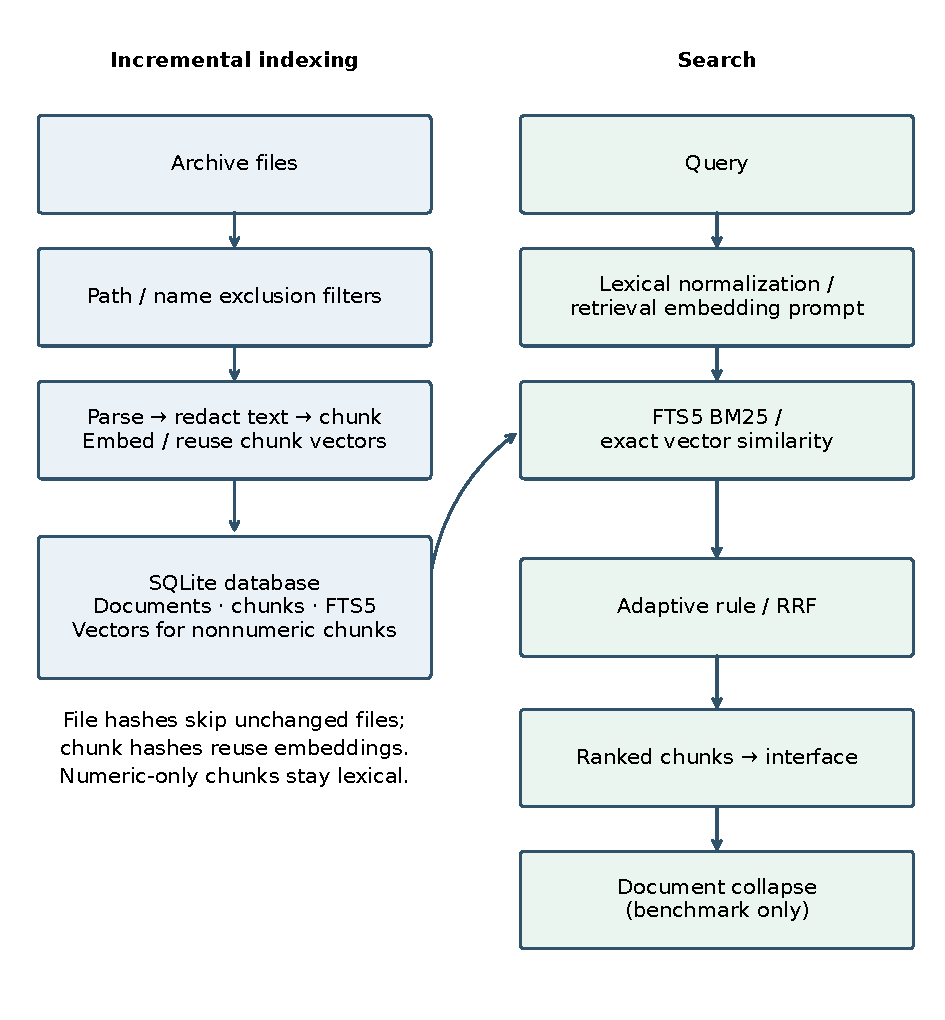
\includegraphics[width=\linewidth]{architecture.pdf}
\caption{Потік даних індексації й пошуку з типовим локальним бекендом. Редагування секретів застосовує відомі текстові шаблони; вміст зображень і звуку так не очищується. Числові фрагменти лишаються доступними лексичному пошуку без векторів. Згортання до документів належить бенчмарку й не входить у таймер запиту.}
\label{fig:architecture}
\end{figure}

\subsection{Лексичний рівень}
Слово --- це послідовність літер і цифр Юнікоду, яку можуть з'єднувати дефіс або апостроф, завдовжки щонайменше два символи, у нижньому регістрі. Чотири символи апострофа, що трапляються в українському тексті (U+2019, U+02BC, U+2018 і зворотний гравіс), до токенізації замінюються на апостроф ASCII, тож \emph{м’ята} і \emph{мʼята} --- одне слово. Стовпець \code{terms} зберігає кожне слово і його нормальні форми з українського та російського аналізаторів pymorphy3. Слово з літерою, що є лише в українській абетці (і, ї, є, ґ), проходить тільки український аналізатор; інші слова --- обидва. Якщо словник знає слово, зберігаються лише словникові нормальні форми; здогадки аналізаторів використовуються тільки для слів, яких не знає жоден словник (ваду, яку виправляє це правило, описано в додатку~\ref{sec:intro-history}).

Ідентифікатори на кшталт \code{36.101}, \code{19.6.0} чи \code{RVZ0014A-2} (послідовності літер і цифр, з'єднані крапками чи скісними рисками, або дефісом перед цифрою) шукаються як точні фрази, тож запит \code{36.109} ніколи не збігається з документом, що містить лише \code{36}. Запит стає виразом FTS5, у якому кожне слово --- диз'юнкція його поверхневої та нормальних форм, слова поєднано через OR, а умову ідентифікатора, якщо вона є, приєднано до слів через AND. Лексичне ранжування --- BM25 у FTS5.

\subsection{Семантичний рівень}
Семантичний рівень використовує EmbeddingGemma~2 через SentenceTransformers: у bfloat16 на GPU (картка моделі попереджає, що float16 погіршує вкладення) і у float32 на CPU. Документи кодуються як \code{title: <назва> | text: <фрагмент>}; запити отримують пошуковий промпт моделі \code{task: search result | query:}, а при пошуку в колекції коду --- \code{task: code retrieval | query:}. Вектори нормуються за L2; 256-вимірний варіант обрізає їх (матрьошкове обрізання) і нормує знову. Зображення, сторінки PDF без текстового шару і кадри відео (один раз на 5~с, не більше 120 на відео) кодуються як зображення в тому самому просторі. Звук передискретизується до 16~кГц і кодується вікнами по 20~с із кроком 15~с; якщо до запису додано файл розшифровки, рядки розшифровки, що перетинаються з вікном, стають його текстом. Сервер llama.cpp із GGUF-збіркою моделі --- необов'язковий суто текстовий бекенд. Семантичний пошук точний: усі вектори тримаються в пам'яті й оцінюються одним добутком матриці на вектор у NumPy, без індексу наближеного пошуку найближчих сусідів.

\subsection{Злиття}
Доступні три режими ранжування: лише лексичний, лише семантичний і гібридний. Типова гібридна стратегія (\sys{adaptive}) дивиться на найкращий лексичний фрагмент. Якщо він містить щонайменше 90\% слів запиту як окремі слова, запит вважається пошуком точної фрази: повертаються лише лексичні результати в порядку BM25, але фрагменти, де слова запиту йдуть по порядку з проміжком до трьох слів, переносяться наперед. Інакше спершу йде семантичне ранжування, а за ним --- лексичні результати, яких у ньому ще немає; без лексичного збігу результат суто семантичний. Альтернативна гібридна стратегія --- злиття за оберненими рангами (reciprocal rank fusion) з $k=60$ (\sys{rrf}). Інтерфейс показує щонайбільше три фрагменти документа і кількість решти; прогони бенчмарку згортають фрагменти до документів (розділ~\ref{sec:method}).

\subsection{Інкрементальна індексація}
Файл пропускається, якщо не змінилися розмір і час зміни, а також якщо не змінився SHA-256; лише інакше його розбирають знову. Вектори фрагментів, геш тексту яких уже збережено, використовуються повторно, тож після правки нотатки заново кодуються тільки змінені фрагменти. Зниклі файли видаляються зі своєї колекції. Фрагменти нотаток і документів, що мають менше 20 літер (номери сторінок, розділові знаки), відкидаються, якщо не всі фрагменти файлу такі короткі; зображення і звук не відкидаються ніколи. Кожен запуск записує звіт про проіндексовані, пропущені й невдалі файли; помилка в одному файлі не зупиняє запуску.

\subsection{Приватність}
Типовий бекенд вкладень обробляє вміст документів локально. Необов'язковий клієнт llama.cpp типово звертається до сервера через петльову адресу; зовнішня адреса у \code{ARCHIVE\_LLAMA\_URL} передає текст до цього вузла. Отже, локальність оброблення залежить від налаштування бекенду. Каталоги \code{.ssh}, \code{.gnupg}, \code{.aws}, \code{.kube}, \code{.password-store}, \code{.docker} і сховища ключів, а також файли, назви яких відповідають шаблонам ключів, сертифікатів, сховищ паролів, файлів оточення й облікових даних (наприклад, \code{*.pem}, \code{*.kdbx}, \code{id\_rsa*}, \code{.env}, \code{*secret*}, \code{*token*}), ніколи не потрапляють до індексу. У проіндексованому тексті блоки приватних ключів PEM, ключі доступу у форматах кількох поширених сервісів (OpenAI, AWS, GitHub, Slack, bearer-токени) та явні присвоєння облікових даних на зразок \code{password=...} замінюються міткою до збереження. Шаблони охоплюють лише відомі формати; це страховка, а не гарантія. Звіт про приховування рахує види і ніколи не зберігає значень.

% Бенчмарк UA-PAR. Кількості з paper/results/corpus_summary.json і маніфесту; правила запитів з paper/guidelines/queries.md.
\section{Бенчмарк UA-PAR}\label{sec:uapar}

\subsection{Джерела і корпус}
\uapar{} відтворює архів дослідника на матеріалі з відкритими ліцензіями українською і російською мовами (ліцензії --- у розділі~\ref{sec:availability}). Корпус має 7\,070 файлів у шести частинах. \emph{Нотатки}: 2\,945 статей Вікіпедії (1\,960 українських, 985 російських) з 25 тем, переважно технічних, серед них антени, радіо, LTE, програмно-визначене радіо, обробка сигналів, мікроконтролери, криптографія, машинне навчання, фізика, історія й література; кожна стаття збережена як нотатка Markdown з рядком джерела. \emph{Документи}: ще 400 статей (260 українських, 140 російських), зверстаних у 133 PDF, 134 DOCX і 133 PPTX, щоб архів мав офісні формати. \emph{Таблиці}: 150 наборів даних data.gov.ua, 100 збережено як CSV і 50 перетворено на XLSX. \emph{Код}: 1\,775 файлів з 30 репозиторіїв GitHub на українську тематику, проіндексованих як колекція коду. \emph{Зображення}: 1\,000 зображень Crossmodal-3600. \emph{Мовлення}: 800 записів FLEURS, 400 українських і 400 російських. Статті зібрано тематичним пошуком збирачем із посторінковою вибіркою і відновленням; для теми SDR не вистачило довгих статей, тож нотаток на 55 менше від запланованих 3\,000, а не доповнено слабко пов'язаними статтями.

Не кожен зібраний файл індексується: archive-index пропускає згенеровані й сторонні файли в репозиторіях, тож повний індекс EG2 містить 6\,054 документи (759 з частини коду) і 96\,908 фрагментів. Суто текстовий індекс E5 містить 4\,137 текстових документів того самого корпусу і жодних зображень чи мовлення; у розділі~\ref{sec:results} показано, що обмеження EG2 тими самими 4\,137 документами змінює його nDCG@10 на $-0{,}0015$.

\subsection{Запити}
Є 200 запитів п'яти категорій із фіксованими квотами: 40 запитів \emph{на відомий документ}, що описують конкретний документ, не цитуючи його назви; 60 \emph{тематичних} запитів, на які можуть відповідати кілька документів; 40 \emph{технічних} запитів з ідентифікаторами, номерами моделей чи стандартами в тому вигляді, як їх пишуть люди; 30 \emph{міжмовних} запитів російською до української цілі або навпаки; і 30 запитів \emph{без відповіді} --- правдоподібних питань про те, чого в корпусі немає, часто з вигаданими номерами моделей. 126 запитів українською і 74 російською. Кожен із 170 запитів з відповіддю написано для однієї цільової нотатки; вона записана, але не є єдиним релевантним документом. Валідатор перевіряє квоти й частки мов, існування кожної цілі, те, що жоден тематичний чи міжмовний запит не має з ціллю спільної послідовності понад п'ять токенів поспіль (жодного копіювання), і те, що кожен запит без відповіді не має жодного лексичного збігу в індексі. Усі 200 запитів проходять перевірку.

Запити написала GPT-6-Luna через Codex CLI за цими правилами. Оскільки автор запитів не має оцінювати власні запити, оцінки GPT ніколи не входять до міток релевантності; вони використовуються лише для порівняння оцінювання, яке не відокремлює самопреференцію від загальної поблажливості (розділ~\ref{sec:results}). Запити без відповіді за побудовою не мають лексичних збігів, тож BM25 нічого на них не повертає; порівняння систем на цих запитах --- це перевірка, чи щільна система колись утримується від відповіді, а не чесне змагання лексичного і щільного пошуку.

\subsection{Оцінювання релевантності}
Пул оцінювання — об'єднання перших десяти документів кожної з десяти систем: 5\,572 пари «запит--документ» для 200 запитів. Окремо перемішані аркуші приховують назви пошукових систем. Суддя бачить запит, назву й початок документа, разом до 1\,200 символів; для аудіозаписів додано транскрипт джерела. Шкала: 0 — не стосується запиту, 1 — частково релевантний, 2 — прямо відповідає на запит. Це оцінки видимого фрагмента, а не результат перегляду повного документа.

Початковий основний суддя — Gemini~3.8 Flash через \code{agy}, пакетами по 50 пар. Gemma~4 12B через Ollama дає основні оцінки для перевірки стійкості висновків; Gemma~4 E4B — додаткові оцінки з відкритими вагами. Запити склала GPT-6-Luna; її оцінки наведено лише для порівняння, до основних і контрольних міток релевантності вони не входять. Усі початкові аркуші збережено. Gemini та Gemma мають спільного постачальника, тому окреме оцінювання не означає незалежності навчальних даних або помилок.

Початкові Gemini та Gemma~4 12B розійшлися на 1\,091 парі. Для варіанта після перегляду окремий прохід Gemini переоцінює ці пари, бачачи обидві початкові оцінки під нейтральними позначеннями A/B зі збалансованим порядком подання. Узгоджені оцінки зберігаються. Це перегляд тією самою моделлю, а не незалежний арбітраж третього судді. Результати пошуку порівнюються за початковими Gemini, початковими Gemma~4 12B та Gemini після перегляду. Основного суддю обрано після перегляду узгодженості й діагностики цільових документів та запитів без відповіді, до поданого сукупного порівняння ефективності систем; попередньої реєстрації цього вибору не було. Завершена перевірка релевантності людиною не заявляється.

Усі 170 запитів із відповіддю мають цільові документи з нотаток; до пулу глибини 10 потрапили 134 цілі. Отже, знаменник діагностики оцінок цільових документів — 134, а не весь набір цілей. Тридцять запитів, позначених як такі, що не мають відповіді, аналізуються окремо.

\subsection{Мультимодальні підмножини}
Пошук зображень і мовлення за текстом оцінюється поза пулом бенчмарку за парами «підпис--зображення» та «транскрипт--запис» із вихідних наборів, без окремо зібраних оцінок релевантності. Для зображень запит --- перший український чи російський підпис зображення в Crossmodal-3600, а правильна відповідь --- це зображення серед усіх 1\,000. Для мовлення запит --- розшифровка речення FLEURS, а правильні відповіді --- записи цього речення; FLEURS n-сторонньо паралельний, тож російська розшифровка може шукати українські записи того самого речення і навпаки. Кожну умову оцінено трьома способами: за аудіовектором запису, за його розшифровкою, закодованою як текст, і за кращим із двох. Коли запит --- розшифровка того самого запису, текстова й комбінована оцінки є верхньою межею, а не результатом пошуку; твердження спираються на умови лише з аудіо і на міжмовні умови.

% Методика виміряного пошуку; невиконані вимірювання ресурсів позначено явно.
\section{Методика оцінювання}\label{sec:method}

\subsection{Системи й одиниця ранжування}
Усі системи використовують одну реалізацію пошуку archive-index з явними перемикачами конфігурації. Порівнюються BM25 без лем і з лемами, повнорозмірна EmbeddingGemma~2, варіант EG2 із 256 вимірами, multilingual-E5, злиття взаємних рангів, адаптивна система та три абляції: без переранжування фраз, обробки ідентифікаторів або фільтра коротких фрагментів. Прогони мають рівень документів: ранг визначає перший знайдений фрагмент документа, наступні його фрагменти згортаються. Для запиту зберігається до 100 документів. Індекс E5 лише текстовий, на відміну від повних індексів EG2; відмінність наборів кандидатів описано як обмеження.

\subsection{Набір запитів і метрики}
Для кожної системи й варіанта суддів середні метрики обчислюються на тих самих 170 запитах із відповіддю з однаковою вагою кожного запиту. Тридцять запитів, позначених як такі, що не мають відповіді, залишаються у файлах релевантності, але не входять до цих середніх; для них окремо наводяться порожня видача й наявність результатів з позитивною оцінкою. Запит із відповіддю, для якого в пулі немає позитивних оцінок, залишається в середньому з нульовою метрикою.

Основна метрика — nDCG@10 із лінійними вагами релевантності 0, 1 і 2, дисконтуванням на $\log_2(i+1)$ для рангу $i$ й нормалізацією за ідеальним ранжуванням оцінених документів. Додаткові метрики — обернений ранг на глибині 10, успіх на глибині 1 і 5 та повнота на глибині 100. У бінарних метриках релевантними вважаються оцінки 1 і 2. Перші десять знайдених документів кожної системи оцінено повністю, проте поза об'єднаним пулом глибини 10 оцінки неповні. Отже, повнота на глибині 100 визначається відносно відомого релевантного пулу, а не всього корпусу. Результати також групуються за категорією й мовою запиту.

\subsection{Невизначеність і порівняння}
Довірчі інтервали середніх метрик і парних середніх різниць отримано процентильним бутстрепом за запитами: 10\,000 перевибірок, початкове зерно 2026. Двобічний парний рандомізаційний тест зі зміною знаків використовує 10\,000 перевибірок і поправку $(b+1)/(10\,000+1)$. Для кожної метрики й варіанта суддів дев'ять порівнянь з повною адаптивною системою утворюють одну сім'ю; p-значення коригуються методом Holm усередині сім'ї з порогом 0,05. Початкове дослідницьке питання про морфологію додатково оцінюється окремо позначеним парним порівнянням BM25 із лемами та без них за nDCG@10; його нескориговане p-значення не входить до сім'ї порівнянь з адаптивною системою. Перетин окремих довірчих інтервалів або відсутність значущої різниці не тлумачаться як еквівалентність.

Для початкової узгодженості суддів наведено лінійно зважену каппу Коена з 95\% інтервалом за 2\,000 бутстреп-перевибірками запитів. Перевибірка запитів, а не окремих пар оцінок зберігає групування всередині запиту. Ці інтервали узгодженості відокремлені від інтервалів метрик пошуку з 10\,000 перевибірками. Для кожного варіанта релевантності наведено ранги систем і зміни попарного порядку; середні, рівні з точністю $10^{-12}$, мають спільний ранг.

\subsection{Відтворюваність і рівні свідчень}
Початкові аркуші оцінок, визначення запитів, маніфест корпусу, пошукові прогони й доступні журнали викликів зафіксовано до обчислення поданого сукупного порівняння ефективності. Маніфест SHA-256 перевіряє ці входи; окремий запис підготовки пов'язує перегляд із початковими розбіжностями та порядком подання. Структуровані відповіді записуються разом з ідентифікаторами моделей, розмов і використанням токенів, коли вони доступні. Після повного перегляду підсумкові мітки замінюють лише оцінки розбіжностей, зберігаючи всі узгоджені оцінки. Таблиці й рисунки генеруються з отриманих JSON-артефактів, а не підтримуються як незалежні числові копії.

Модульні й інтеграційні перевірки встановлюють поведінку реалізації; публічний бенчмарк дає свідчення пошуку за оцінками моделей; окремі мультимодальні експерименти використовують мітки джерельних наборів даних. Ці типи свідчень не замінюють перевірку релевантності людиною чи вимірювання під час експлуатації.

\subsection{Вимірювання ресурсів}
Затримка запиту --- це час кодування запиту та пошуку фрагментів в оцінювальній обв'язці, включно з лексичним і семантичним пошуком та злиттям, із межею 400 фрагментів-кандидатів. Таймер зупиняється до згортання до документів і визначення шляхів; це не наскрізна затримка інтерфейсу. Кожна система відповідає на всі 200 запитів один раз для розігріву і ще раз під вимірюванням, в одному процесі, спершу з видимим GPU, а потім з порожньою змінною \code{CUDA\_VISIBLE\_DEVICES} (моделі вкладень тоді працюють на CPU у float32). Під час кожного виміряного проходу обв'язка записує використання CPU по ядрах із \code{/proc/stat}, секунди CPU кожного потоку процесу з \code{/proc/self/task}, зміну лічильників переривань по ядрах із \code{/proc/interrupts}, піковий резидентний розмір і пам'ять GPU, яку \code{nvidia-smi} опитує кожні 0,2~с. Машина працювала у звичайному робочому сеансі; середнє навантаження за хвилину перед кожним кроком записано в журнал вимірювань.

Вартість індексації виміряно на фіксованій випадковій вибірці корпусу (зерно 2026: 300 нотаток, 40 документів, 15 таблиць, 60 зображень і 60 записів), яку команда \code{archive} індексує в порожню базу з GPU. Для CPU взято п’яту частину за кількістю: 60 нотаток, 8 документів, 3 таблиці, 12 зображень і 12 записів. Вибірки відрізняються розміром та складом, тому співвідношення їхнього повного часу не є парною оцінкою прискорення CPU/GPU. Розміри чотирьох повних індексів бенчмарку подано такими, як їх побудовано.

Для квантування текстові фрагменти повного індексу (84\,788 векторизованих рядків текстових колекцій) кодуються заново GGUF-збірками EmbeddingGemma~2 (f16, Q8\_0, Q4\_K\_M), які обслуговує llama.cpp із середнім пулінгом і тими самими префіксами \code{title: \ldots{} | text: \ldots}; запити мають той самий пошуковий промпт. Щільний пошук із кожною збіркою йде по 4\,137 текстових документах і порівнюється з моделлю SentenceTransformers у bfloat16 на тих самих документах (\sys{dense\_eg2\_text}) з тими самими мітками. Документи, які квантований прогін приносить у першу десятку, але яких не бачив жоден суддя, вважаються нерелевантними, і їхню частку подано. Текстові колекції містять 21 рядок сторінок PDF, які повна модель кодує як зображення. GGUF натомість кодує збережений для них текст (загалом 485 символів); 84\,767 рядків мають текстовий вхід. Отже, однакові документи-кандидати не означають однакової модальності входу для кожного фрагмента, і порівняння не ізолює лише квантування.

Масштабування точного щільного пошуку виміряно поза archive-index на колекціях, вирощених із 86\,726 справжніх векторів EG2 до $10^5$, $3\cdot10^5$, $10^6$ і $2\cdot10^6$ векторів; додані вектори --- зашумлені копії справжніх (гаусів шум, $\sigma=0{,}05$, з повторним нормуванням), тож колекції синтетичні. Кожен із 200 векторів запитів UA-PAR шукається окремо оптимізованим точним вибором першої десятки в NumPy (добуток матриці й \code{argpartition}), точним індексом Faiss та індексом HNSW ($M=32$, глибина побудови 200, глибина пошуку 64 і 256). Послідовний додатковий прогін викликає справжній метод ранжування векторів archive-index на тих самих матрицях: збирання кандидатів, повне \code{argsort} і побудову 400 кортежів результатів, без перевірки версії кешу SQLite. Це відокремлює оптимізований еталон від розгорнутого алгоритму. Повнота@10 HNSW рахує збіги ідентифікаторів векторів із NumPy; однакові оцінки й різниці обчислень не зараховуються як еквівалентні ідентифікатори. Окремо перевіряються збіг точних ранжувань Faiss і NumPy та частка результатів Faiss з оцінкою не нижче десятої еталонної з допуском $10^{-6}$.

\subsection{Програмне й апаратне забезпечення}
Усі вимірювання виконано на одному ноутбуці: Intel Core i9-14900HX (32 логічні процесори), 31~ГіБ ОЗП, NVIDIA GeForce RTX 4060 Laptop GPU з 8~ГБ, Linux 7.0. Програмне забезпечення: Python 3.13.14, PyTorch 2.14.1, Transformers 5.19.0, SentenceTransformers 6.1.0, NumPy 2.5.4, SQLite 3.53.1, pymorphy3 2.0.6, ir-measures 0.4.3, llama.cpp коміт \code{8bb3cf0} і Faiss 1.15.1 в окремому середовищі для експерименту масштабування. Повний перелік збережено в \code{efficiency.json}.

% Таблиці й рисунки з результатів; інтерпретацію додано після завершення перегляду.
\section{Результати}\label{sec:results}
% Generated from primary=gemini_reviewed; see ../manifest.json for source SHA-256.
\newif\ifpaperlatency
\paperlatencytrue
\newif\ifpaperindexing
\paperindexingtrue
\newif\ifpapergguf
\papergguftrue
\newif\ifpaperann
\paperanntrue
\newif\ifpaperfield
\paperfieldtrue
\newif\ifpaperextension
\paperextensiontrue
\newif\ifpaperextensionunique
\paperextensionuniquetrue


\subsection{Пошук і стійкість до вибору судді}
Таблиця~\ref{tab:retrieval} містить усі десять систем на однаковому наборі запитів із відповіддю. Довірчі інтервали описують варіацію за запитами за наведених міток, але не невизначеність самих міток. Таблиця~\ref{tab:judge-sensitivity} та рисунок~\ref{fig:judge-sensitivity} зберігають початкові й переглянутий варіанти. Перегляд виконує та сама модель Gemini; Gemini та Gemma мають спільного постачальника.

E5 має найвище середнє nDCG@10 за всіма трьома основними варіантами релевантності. Її перевага над adaptive не досягає порога 0,05 після поправки Holm за жодного варіанта; це не доводить еквівалентності. Adaptive перевершує обидва варіанти BM25 за основною метрикою після корекції, але статистично виявленої переваги над окремою EG2 або RRF немає. Вимкнення переранжування фраз не змінює оцінених метрик; відмінності інших абляцій адаптивної системи за nDCG@10 малі й статистично не виявлені на цьому наборі запитів. Ці результати не підтверджують загального твердження про перевагу адаптивного злиття над пошуком лише за векторами.

Лематизація підвищує середнє nDCG@10 BM25 за всіх трьох варіантів. Окремо наведене парне морфологічне порівняння підтримує різницю за початковими та переглянутими оцінками Gemini, тоді як за оцінками Gemma~4 12B інтервал охоплює нуль. Отже, сила висновку про морфологію залежить від оцінювання релевантності. Перегляд тією самою моделлю змінює 334 із 5\,572 початкових оцінок Gemini; усі 4\,481 початково узгоджені пари зберігаються.

\begin{table}[p]
\centering
\caption{Пошук документів за 170 запитами із відповіддю. Середні та 95\% бутстреп-інтервали за запитами відповідають оцінкам Gemini після перегляду розбіжностей тією самою моделлю. Дві частини зберігають усі п'ять метрик. Знак \textdagger{} позначає парну різницю з adaptive за скоригованого Holm $p<0.05$, не обов'язково поліпшення. R@100 визначено відносно пулу. E5 має менший текстовий набір кандидатів.}
\label{tab:retrieval}
% Generated from primary=gemini_reviewed; see ../manifest.json for source SHA-256.
% Means with 95% bootstrap CI; n=170. R@100 is pool-relative under incomplete judgments. Significance: paired comparison against adaptive only, \(p_{\mathrm{Holm}}<0.05\).
\begingroup\small\setlength{\tabcolsep}{4pt}\renewcommand{\arraystretch}{1.3}
\noindent\begin{tabularx}{\linewidth}{@{}l*{3}{>{\centering\arraybackslash}X}@{}}
\toprule
Система & nDCG@10 & R@100\textsuperscript{pool} & RR@10 \\
\midrule
bm25\_plain & \shortstack{0.450\textsuperscript{\textdagger} \\ {\footnotesize[0.413, 0.487]}} & \shortstack{0.648\textsuperscript{\textdagger} \\ {\footnotesize[0.611, 0.685]}} & \shortstack{0.738\textsuperscript{\textdagger} \\ {\footnotesize[0.682, 0.790]}} \\
bm25\_lemma & \shortstack{0.482\textsuperscript{\textdagger} \\ {\footnotesize[0.446, 0.518]}} & \shortstack{0.724\textsuperscript{\textdagger} \\ {\footnotesize[0.693, 0.755]}} & \shortstack{0.753\textsuperscript{\textdagger} \\ {\footnotesize[0.701, 0.802]}} \\
dense\_eg2 & \shortstack{0.633 \\ {\footnotesize[0.601, 0.664]}} & \shortstack{0.911 \\ {\footnotesize[0.890, 0.930]}} & \shortstack{0.872 \\ {\footnotesize[0.832, 0.910]}} \\
dense\_e5 & \shortstack{0.674 \\ {\footnotesize[0.647, 0.700]}} & \shortstack{0.880 \\ {\footnotesize[0.853, 0.906]}} & \shortstack{0.927 \\ {\footnotesize[0.894, 0.956]}} \\
rrf & \shortstack{0.630 \\ {\footnotesize[0.601, 0.660]}} & \shortstack{0.960\textsuperscript{\textdagger} \\ {\footnotesize[0.946, 0.972]}} & \shortstack{0.873 \\ {\footnotesize[0.835, 0.910]}} \\
adaptive & \shortstack{0.629 \\ {\footnotesize[0.596, 0.660]}} & \shortstack{0.908 \\ {\footnotesize[0.887, 0.928]}} & \shortstack{0.866 \\ {\footnotesize[0.826, 0.905]}} \\
adaptive-phrase & \shortstack{0.629 \\ {\footnotesize[0.596, 0.660]}} & \shortstack{0.908 \\ {\footnotesize[0.887, 0.928]}} & \shortstack{0.866 \\ {\footnotesize[0.826, 0.905]}} \\
adaptive-ident & \shortstack{0.629 \\ {\footnotesize[0.597, 0.661]}} & \shortstack{0.912 \\ {\footnotesize[0.892, 0.931]}} & \shortstack{0.866 \\ {\footnotesize[0.826, 0.905]}} \\
adaptive-short & \shortstack{0.629 \\ {\footnotesize[0.597, 0.660]}} & \shortstack{0.908 \\ {\footnotesize[0.887, 0.928]}} & \shortstack{0.866 \\ {\footnotesize[0.826, 0.905]}} \\
dense\_eg2\_256 & \shortstack{0.611 \\ {\footnotesize[0.577, 0.643]}} & \shortstack{0.888\textsuperscript{\textdagger} \\ {\footnotesize[0.863, 0.911]}} & \shortstack{0.873 \\ {\footnotesize[0.830, 0.913]}} \\
\bottomrule
\end{tabularx}\endgroup

\par\medskip
% Means with 95% bootstrap CI; n=170. R@100 is pool-relative under incomplete judgments. Significance: paired comparison against adaptive only, \(p_{\mathrm{Holm}}<0.05\).
\begingroup\small\setlength{\tabcolsep}{4pt}\renewcommand{\arraystretch}{1.3}
\noindent\begin{tabularx}{\linewidth}{@{}l*{2}{>{\centering\arraybackslash}X}@{}}
\toprule
Система & Success@1 & Success@5 \\
\midrule
bm25\_plain & \shortstack{0.635\textsuperscript{\textdagger} \\ {\footnotesize[0.559, 0.706]}} & \shortstack{0.876\textsuperscript{\textdagger} \\ {\footnotesize[0.824, 0.924]}} \\
bm25\_lemma & \shortstack{0.624\textsuperscript{\textdagger} \\ {\footnotesize[0.547, 0.694]}} & \shortstack{0.929 \\ {\footnotesize[0.888, 0.965]}} \\
dense\_eg2 & \shortstack{0.794 \\ {\footnotesize[0.729, 0.853]}} & \shortstack{0.971 \\ {\footnotesize[0.941, 0.994]}} \\
dense\_e5 & \shortstack{0.876 \\ {\footnotesize[0.824, 0.924]}} & \shortstack{0.988 \\ {\footnotesize[0.971, 1.000]}} \\
rrf & \shortstack{0.788 \\ {\footnotesize[0.724, 0.847]}} & \shortstack{0.976 \\ {\footnotesize[0.953, 0.994]}} \\
adaptive & \shortstack{0.782 \\ {\footnotesize[0.718, 0.841]}} & \shortstack{0.971 \\ {\footnotesize[0.941, 0.994]}} \\
adaptive-phrase & \shortstack{0.782 \\ {\footnotesize[0.718, 0.841]}} & \shortstack{0.971 \\ {\footnotesize[0.941, 0.994]}} \\
adaptive-ident & \shortstack{0.782 \\ {\footnotesize[0.718, 0.841]}} & \shortstack{0.971 \\ {\footnotesize[0.941, 0.994]}} \\
adaptive-short & \shortstack{0.782 \\ {\footnotesize[0.718, 0.841]}} & \shortstack{0.971 \\ {\footnotesize[0.941, 0.994]}} \\
dense\_eg2\_256 & \shortstack{0.818 \\ {\footnotesize[0.759, 0.871]}} & \shortstack{0.953 \\ {\footnotesize[0.918, 0.982]}} \\
\bottomrule
\end{tabularx}\endgroup

\par\smallskip
{\footnotesize \textdagger: p\textsubscript{Holm}<0.05, adaptive; R@100: відносно пулу.}

\end{table}

\begin{table}[p]
\centering
\caption{Стійкість nDCG@10 до оцінювання релевантності. Початкові оцінки Gemini та Gemma~4 12B збережено; варіант після перегляду змінює лише їхні розбіжності. Усі варіанти використовують ті самі зафіксовані прогони та 170 запитів. Оцінки GPT до цього порівняння не входять.}
\label{tab:judge-sensitivity}
% Generated from primary=gemini_reviewed; see ../manifest.json for source SHA-256.
% nDCG@10 with 95% bootstrap CI. Gemini reviewed is a within-model review. Gemini/Gemma12 share a provider family. No GPT or E4B in this principal comparison.
\begingroup\small\setlength{\tabcolsep}{4pt}\renewcommand{\arraystretch}{1.3}
\noindent\begin{tabularx}{\linewidth}{@{}l*{3}{>{\centering\arraybackslash}X}@{}}
\toprule
Система & Gemini початкові & Gemma12 початкові & Gemini переглянуті \\
\midrule
bm25\_plain & \shortstack{0.453 \\ {\footnotesize[0.416, 0.491]}} & \shortstack{0.500 \\ {\footnotesize[0.462, 0.536]}} & \shortstack{0.450 \\ {\footnotesize[0.413, 0.487]}} \\
bm25\_lemma & \shortstack{0.489 \\ {\footnotesize[0.453, 0.526]}} & \shortstack{0.519 \\ {\footnotesize[0.482, 0.554]}} & \shortstack{0.482 \\ {\footnotesize[0.446, 0.518]}} \\
dense\_eg2 & \shortstack{0.644 \\ {\footnotesize[0.613, 0.674]}} & \shortstack{0.681 \\ {\footnotesize[0.652, 0.709]}} & \shortstack{0.633 \\ {\footnotesize[0.601, 0.664]}} \\
dense\_e5 & \shortstack{0.685 \\ {\footnotesize[0.657, 0.711]}} & \shortstack{0.698 \\ {\footnotesize[0.671, 0.725]}} & \shortstack{0.674 \\ {\footnotesize[0.647, 0.700]}} \\
rrf & \shortstack{0.641 \\ {\footnotesize[0.612, 0.669]}} & \shortstack{0.665 \\ {\footnotesize[0.636, 0.694]}} & \shortstack{0.630 \\ {\footnotesize[0.601, 0.660]}} \\
adaptive & \shortstack{0.639 \\ {\footnotesize[0.608, 0.669]}} & \shortstack{0.675 \\ {\footnotesize[0.647, 0.703]}} & \shortstack{0.629 \\ {\footnotesize[0.596, 0.660]}} \\
adaptive-phrase & \shortstack{0.639 \\ {\footnotesize[0.608, 0.669]}} & \shortstack{0.675 \\ {\footnotesize[0.647, 0.703]}} & \shortstack{0.629 \\ {\footnotesize[0.596, 0.660]}} \\
adaptive-ident & \shortstack{0.639 \\ {\footnotesize[0.608, 0.669]}} & \shortstack{0.676 \\ {\footnotesize[0.648, 0.704]}} & \shortstack{0.629 \\ {\footnotesize[0.597, 0.661]}} \\
adaptive-short & \shortstack{0.639 \\ {\footnotesize[0.608, 0.669]}} & \shortstack{0.675 \\ {\footnotesize[0.647, 0.703]}} & \shortstack{0.629 \\ {\footnotesize[0.597, 0.660]}} \\
dense\_eg2\_256 & \shortstack{0.622 \\ {\footnotesize[0.589, 0.654]}} & \shortstack{0.665 \\ {\footnotesize[0.633, 0.696]}} & \shortstack{0.611 \\ {\footnotesize[0.577, 0.643]}} \\
\bottomrule
\end{tabularx}\endgroup

\end{table}

\begin{figure}[p]
\centering
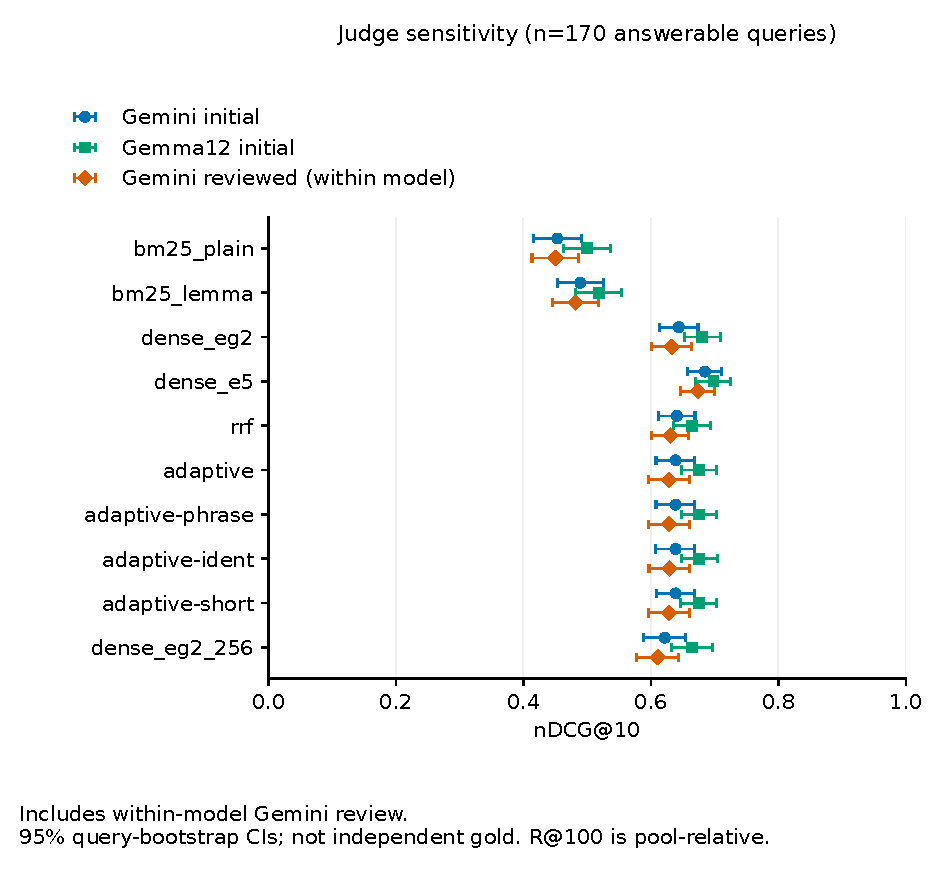
\includegraphics[width=\linewidth]{judge_sensitivity.pdf}
\caption{Метрики систем і 95\% бутстреп-інтервали за запитами для різних варіантів релевантності. Порівняння окремих інтервалів не замінює парних статистичних тестів.}
\label{fig:judge-sensitivity}
\end{figure}

\begin{figure}[p]
\centering
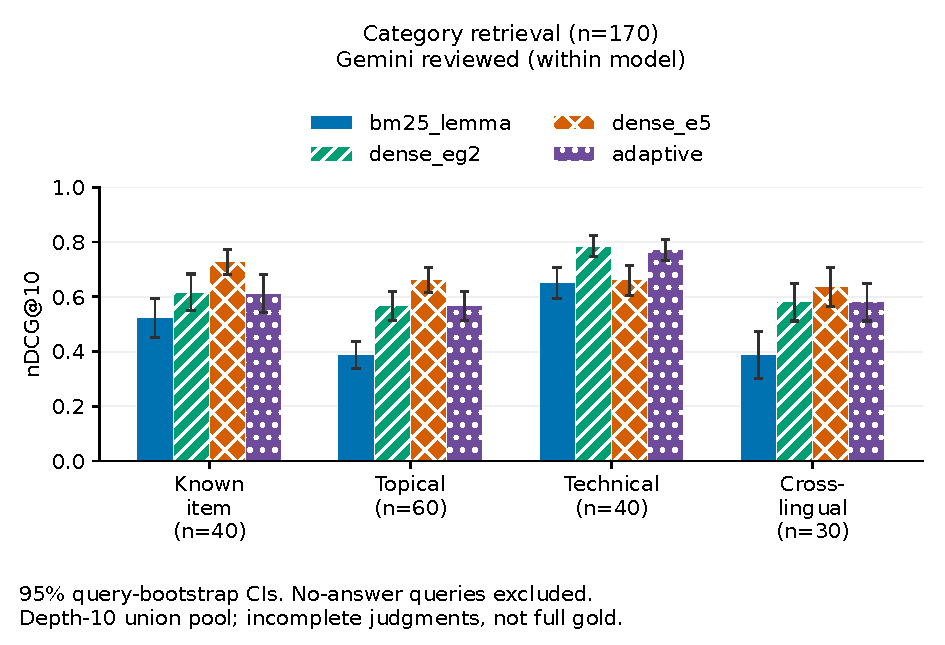
\includegraphics[width=\linewidth]{category_ndcg.pdf}
\caption{nDCG@10 за категоріями запитів для чотирьох основних систем за основного варіанта релевантності. Кожна категорія має власний бутстреп-інтервал. Запити без відповіді виключено.}
\label{fig:categories}
\end{figure}

\subsection{Контролі}
\paragraph{Множина кандидатів.} E5 шукає серед 4\,137 текстових документів; повний індекс EG2 містить 6\,054 документи, зокрема медіа. Обмеження EG2 тими самими 4\,137 текстовими документами (\sys{dense\_eg2\_text}) змінює його nDCG@10 на $-0{,}0015$ з переглянутими мітками Gemini (з 0,633 до 0,631); 0,29\% документів його першої десятки не було в оціненому пулі. Парна різниця EG2$_{\mathrm{text}}-{}$E5 становить $-0{,}042$ nDCG@10 (95\% ДІ від $-0{,}078$ до $-0{,}006$, некоригований $p=0{,}018$) з переглянутими мітками Gemini і $-0{,}019$ (від $-0{,}052$ до $0{,}014$, $p=0{,}26$) з мітками Gemma~4 12B (табл.~\ref{tab:encoder-control}). Отже, обмеження кандидатів мало змінює точкову оцінку в цьому контролі, а статистична підтримка різниці енкодерів залежить від міток. Ці дослідницькі порівняння мають некориговані p-значення та неповний пул оцінок.

\begin{table}[p]
\centering
\caption{E5 проти EG2 на тих самих 4\,137 текстових документах. $\Delta$ --- парна різниця від E5 з 95\% бутстреп-інтервалом за запитами і некоригованим $p$ знакового перестановкового тесту; неоцінені документи вважаються нерелевантними, їхню частку подано.}
\label{tab:encoder-control}
% Generated from primary=gemini_reviewed; see ../manifest.json for source SHA-256.
\noindent\textbf{Gemini reviewed}
\par\smallskip
% E5 against EG2 on the same 4137 text documents; source encoder_control.json
\begingroup\small\setlength{\tabcolsep}{4pt}\renewcommand{\arraystretch}{1.3}
\noindent\begin{tabularx}{\linewidth}{@{}l*{4}{>{\centering\arraybackslash}X}@{}}
\toprule
Система & nDCG@10 & $\Delta$ [95\% ДІ] vs E5 & p & Неоцінені@10 \\
\midrule
\sys{dense\_e5} & 0.674 & -- & -- & 0.000 \\
\sys{dense\_eg2} & 0.633 & \shortstack{-0.041 \\ {\footnotesize[-0.077, -0.005]}} & 0.023 & 0.000 \\
\sys{dense\_eg2\_text} & 0.631 & \shortstack{-0.042 \\ {\footnotesize[-0.078, -0.006]}} & 0.018 & 0.003 \\
\bottomrule
\end{tabularx}\endgroup

\par\medskip
\noindent\textbf{Gemini initial}
\par\smallskip
% E5 against EG2 on the same 4137 text documents; source encoder_control.json
\begingroup\small\setlength{\tabcolsep}{4pt}\renewcommand{\arraystretch}{1.3}
\noindent\begin{tabularx}{\linewidth}{@{}l*{4}{>{\centering\arraybackslash}X}@{}}
\toprule
Система & nDCG@10 & $\Delta$ [95\% ДІ] vs E5 & p & Неоцінені@10 \\
\midrule
\sys{dense\_e5} & 0.685 & -- & -- & 0.000 \\
\sys{dense\_eg2} & 0.644 & \shortstack{-0.041 \\ {\footnotesize[-0.075, -0.007]}} & 0.020 & 0.000 \\
\sys{dense\_eg2\_text} & 0.642 & \shortstack{-0.042 \\ {\footnotesize[-0.077, -0.009]}} & 0.014 & 0.003 \\
\bottomrule
\end{tabularx}\endgroup

\par\medskip
\noindent\textbf{Gemma 12B initial}
\par\smallskip
% E5 against EG2 on the same 4137 text documents; source encoder_control.json
\begingroup\small\setlength{\tabcolsep}{4pt}\renewcommand{\arraystretch}{1.3}
\noindent\begin{tabularx}{\linewidth}{@{}l*{4}{>{\centering\arraybackslash}X}@{}}
\toprule
Система & nDCG@10 & $\Delta$ [95\% ДІ] vs E5 & p & Неоцінені@10 \\
\midrule
\sys{dense\_e5} & 0.698 & -- & -- & 0.000 \\
\sys{dense\_eg2} & 0.681 & \shortstack{-0.018 \\ {\footnotesize[-0.050, +0.015]}} & 0.285 & 0.000 \\
\sys{dense\_eg2\_text} & 0.680 & \shortstack{-0.019 \\ {\footnotesize[-0.052, +0.014]}} & 0.258 & 0.003 \\
\bottomrule
\end{tabularx}\endgroup

\end{table}

\paragraph{Покриття цілими словами.} Перевірка точної фрази в адаптивному правилі рахувала підрядки (додаток~\ref{sec:intro-history}). З виправленим правилом перша десятка змінюється для одного запиту з 200 у кожному адаптивному варіанті, а nDCG@10 адаптивної системи змінюється з 0,629 до 0,627 (переглянуті Gemini), з 0,639 до 0,637 (початкові Gemini) і лишається 0,675 (Gemma~4 12B). Зафіксовані основні результати збережено; виправлена точкова оцінка не створює переваги адаптивного методу над щільним EG2.

\subsection{Судді}
Табл.~\ref{tab:judge-checks} показує оцінки на всьому пулі та на двох підмножинах із очікуваннями, заданими побудовою: цільових документах у пулі й парах запитів, позначених безвідповідними. Ці очікування не є незалежними людськими мітками. Табл.~\ref{tab:judge-agreement} подає попарну узгодженість. Gemini, дві моделі Gemma і GPT-6-Luna узгоджуються з лінійно зваженою $\kappa$ від 0,535 до 0,652. Gemini ставить оцінку~2 цільовому документу запиту з відповіддю у 85,8\% зі 134 цілей у пулі, Gemma~4 12B --- у 67,2\%: більша модель Gemma загалом найкраще узгоджується з Gemini, але рідко ставить повний бал. На 708 парах запитів без відповіді Gemini, Gemma~4 12B і Gemma~4 E4B ставлять 0 у 90,4\%, 91,2\% і 93,5\% пар.

GPT-6-Luna, яка писала запити, --- найпоблажливіший суддя: її середня оцінка 0,633 проти 0,421--0,447 в інших суддів, і вона ставить додатну оцінку 24,3\% пар запитів без відповіді проти 6,5--9,6\% в інших. Її оцінки в середньому на 0,19--0,21 вищі, ніж у кожного іншого судді. Це узгоджується із самопреференцією автора запитів, але загальна поблажливість дала б ту саму картину. Наявне порівняння не розрізняє цих пояснень. Оцінки GPT не входять до жодних міток релевантності.

\begin{table}[p]
\centering
\caption{Судді на 5\,572 парах пулу: середня оцінка, кількість оцінок і перевірки за побудовою (частка цілей запитів з відповіддю в пулі з оцінкою 2; частка пар запитів без відповіді з оцінкою 0).}
\label{tab:judge-checks}
% Generated from primary=gemini_reviewed; see ../manifest.json for source SHA-256.
% grades on the whole pool and known-answer checks; source judges.json
\begingroup\small\setlength{\tabcolsep}{4pt}\renewcommand{\arraystretch}{1.3}
\noindent\begin{tabularx}{\linewidth}{@{}l*{5}{>{\centering\arraybackslash}X}@{}}
\toprule
Суддя & Пари & Середня оцінка & 0 / 1 / 2 & Ціль = 2, \% & Без відповіді = 0, \% \\
\midrule
Gemini 3.8 Flash & 5\,572 & 0.421 & 3\,522 / 1\,756 / 294 & 85.8 (n=134) & 90.4 (n=708) \\
Gemma 4 12B & 5\,572 & 0.447 & 3\,316 / 2\,024 / 232 & 67.2 (n=134) & 91.2 (n=708) \\
Gemma 4 E4B & 5\,572 & 0.438 & 3\,519 / 1\,665 / 388 & 74.6 (n=134) & 93.5 (n=708) \\
GPT-6-Luna & 5\,572 & 0.633 & 2\,554 / 2\,510 / 508 & 91.8 (n=134) & 75.7 (n=708) \\
\bottomrule
\end{tabularx}\endgroup

\end{table}

\begin{table}[p]
\centering
\caption{Попарна узгодженість суддів на тих самих 5\,572 парах: лінійно зважена $\kappa$ Коена з 95\% інтервалом за 2\,000 бутстреп-вибірками запитів, точний збіг і середня різниця оцінок.}
\label{tab:judge-agreement}
% Generated from primary=gemini_reviewed; see ../manifest.json for source SHA-256.
% linear-weighted kappa, CI by resampling queries; source judges.json
\begingroup\small\setlength{\tabcolsep}{4pt}\renewcommand{\arraystretch}{1.3}
\noindent\begin{tabularx}{\linewidth}{@{}l*{4}{>{\centering\arraybackslash}X}@{}}
\toprule
Судді & Пари & Зважена $\kappa$ [95\% ДІ] & Точний збіг & Середня A$-$B \\
\midrule
Gemini 3.8 Flash – Gemma 4 12B & 5\,572 & 0.652 [0.625, 0.677] & 0.804 & -0.026 \\
Gemini 3.8 Flash – Gemma 4 E4B & 5\,572 & 0.591 [0.559, 0.622] & 0.768 & -0.017 \\
Gemini 3.8 Flash – GPT-6-Luna & 5\,572 & 0.621 [0.595, 0.644] & 0.759 & -0.212 \\
Gemma 4 12B – Gemma 4 E4B & 5\,572 & 0.650 [0.625, 0.674] & 0.799 & +0.008 \\
Gemma 4 12B – GPT-6-Luna & 5\,572 & 0.586 [0.559, 0.612] & 0.741 & -0.186 \\
Gemma 4 E4B – GPT-6-Luna & 5\,572 & 0.535 [0.506, 0.564] & 0.700 & -0.195 \\
\bottomrule
\end{tabularx}\endgroup

\end{table}

\subsection{Зображення й мовлення}
Таблиця~\ref{tab:multimodal} містить окремі завдання пошуку зображень за підписами та мовлення за транскриптами. Для цих точкових оцінок довірчі інтервали не обчислено. Одномовний текстовий режим мовлення використовує той самий транскрипт як запит та індексований текст; отже, це оцінка верхньої межі, а не реалістичний пошук за перефразованим запитом. Міжмовні запити — паралельні транскрипти джерельних даних, які також не представляють довільний розмовний пошук аудіо.

\begin{table}[p]
\centering
\caption{Окремі мультимодальні завдання з мітками джерела: кількість запитів і кандидатів, потім точкові оцінки. Довірчі інтервали не вигадуються. Режим text для мовлення індексує транскрипт; режим both поєднує транскрипт та аудіо.}
\label{tab:multimodal}
% Generated from primary=gemini_reviewed; see ../manifest.json for source SHA-256.
% Separate multimodal tasks; confidence intervals unavailable in source (not fabricated).
\begingroup\small\setlength{\tabcolsep}{4pt}\renewcommand{\arraystretch}{1.3}
\noindent\begin{tabularx}{\linewidth}{@{}l*{2}{>{\centering\arraybackslash}X}@{}}
\toprule
Режим & Запити & Об’єкти \\
\midrule
Зображення / ru & 1000 & 1000 \\
Зображення / uk & 1000 & 1000 \\
Мовлення / ru->ru / аудіо & 265 & 400 \\
Мовлення / ru->ru / обидва & 265 & 400 \\
Мовлення / ru->ru / текст & 265 & 400 \\
Мовлення / ru->uk / аудіо & 194 & 400 \\
Мовлення / ru->uk / обидва & 194 & 400 \\
Мовлення / ru->uk / текст & 194 & 400 \\
Мовлення / uk->ru / аудіо & 194 & 400 \\
Мовлення / uk->ru / обидва & 194 & 400 \\
Мовлення / uk->ru / текст & 194 & 400 \\
Мовлення / uk->uk / аудіо & 262 & 400 \\
Мовлення / uk->uk / обидва & 262 & 400 \\
Мовлення / uk->uk / текст & 262 & 400 \\
\bottomrule
\end{tabularx}\endgroup

\par\medskip
% Point estimates only; confidence intervals unavailable. Recall is task-specific.
\begingroup\small\setlength{\tabcolsep}{4pt}\renewcommand{\arraystretch}{1.3}
\noindent\begin{tabularx}{\linewidth}{@{}l*{4}{>{\centering\arraybackslash}X}@{}}
\toprule
Режим & recall@1 & recall@5 & recall@10 & mrr \\
\midrule
Зображення / ru & 0.889 & 0.983 & 0.994 & 0.932 \\
Зображення / uk & 0.857 & 0.977 & 0.986 & 0.909 \\
Мовлення / ru->ru / аудіо & 0.996 & 1.000 & 1.000 & 0.997 \\
Мовлення / ru->ru / обидва & 1.000 & 1.000 & 1.000 & 1.000 \\
Мовлення / ru->ru / текст & 1.000 & 1.000 & 1.000 & 1.000 \\
Мовлення / ru->uk / аудіо & 0.985 & 1.000 & 1.000 & 0.991 \\
Мовлення / ru->uk / обидва & 1.000 & 1.000 & 1.000 & 1.000 \\
Мовлення / ru->uk / текст & 1.000 & 1.000 & 1.000 & 1.000 \\
Мовлення / uk->ru / аудіо & 0.985 & 1.000 & 1.000 & 0.990 \\
Мовлення / uk->ru / обидва & 1.000 & 1.000 & 1.000 & 1.000 \\
Мовлення / uk->ru / текст & 1.000 & 1.000 & 1.000 & 1.000 \\
Мовлення / uk->uk / аудіо & 0.996 & 1.000 & 1.000 & 0.997 \\
Мовлення / uk->uk / обидва & 1.000 & 1.000 & 1.000 & 1.000 \\
Мовлення / uk->uk / текст & 1.000 & 1.000 & 1.000 & 1.000 \\
\bottomrule
\end{tabularx}\endgroup

\end{table}

\subsection{Затримка й індексування}
\ifpaperlatency
Табл.~\ref{tab:latency} подає затримку розігрітих систем на тих самих 200 запитах. Це час оцінювального стенда на одному ноутбуці, а не гарантія часу інтерактивної відповіді. Моделі залишаються завантаженими між системами, тому приріст загальної пам’яті GPU від базового рівня не є окремим обсягом пам’яті відповідної системи.
\begin{table}[p]
\centering
\caption{Затримка розігрітого запиту в мілісекундах: p50 і p95 на GPU та CPU. VRAM --- загальний приріст пам’яті пристрою від базового рівня етапу; попередні моделі залишаються в пам’яті.}
\label{tab:latency}
% Generated from primary=gemini_reviewed; see ../manifest.json for source SHA-256.
% per-query latency in ms (query embedding and chunk search; document collapse excluded); source efficiency.json
\begingroup\small\setlength{\tabcolsep}{4pt}\renewcommand{\arraystretch}{1.3}
\noindent\begin{tabularx}{\linewidth}{@{}l*{5}{>{\centering\arraybackslash}X}@{}}
\toprule
Система & GPU p50 & GPU p95 & CPU p50 & CPU p95 & VRAM +МіБ \\
\midrule
\sys{bm25\_plain} & 12.3 & 41.6 & 13.8 & 48.0 & 0 \\
\sys{bm25\_lemma} & 19.9 & 64.1 & 19.9 & 62.4 & 0 \\
\sys{dense\_eg2} & 137.9 & 189.4 & 218.3 & 261.5 & 1592 \\
\sys{dense\_eg2\_256} & 67.2 & 79.5 & 185.8 & 212.9 & 0 \\
\sys{dense\_e5} & 93.1 & 117.1 & 217.2 & 254.5 & 2130 \\
\sys{rrf} & 132.5 & 177.4 & 266.8 & 362.1 & 2 \\
\sys{adaptive} & 134.7 & 186.7 & 230.4 & 286.3 & 0 \\
\bottomrule
\end{tabularx}\endgroup

\end{table}
\begin{figure}[p]
\centering
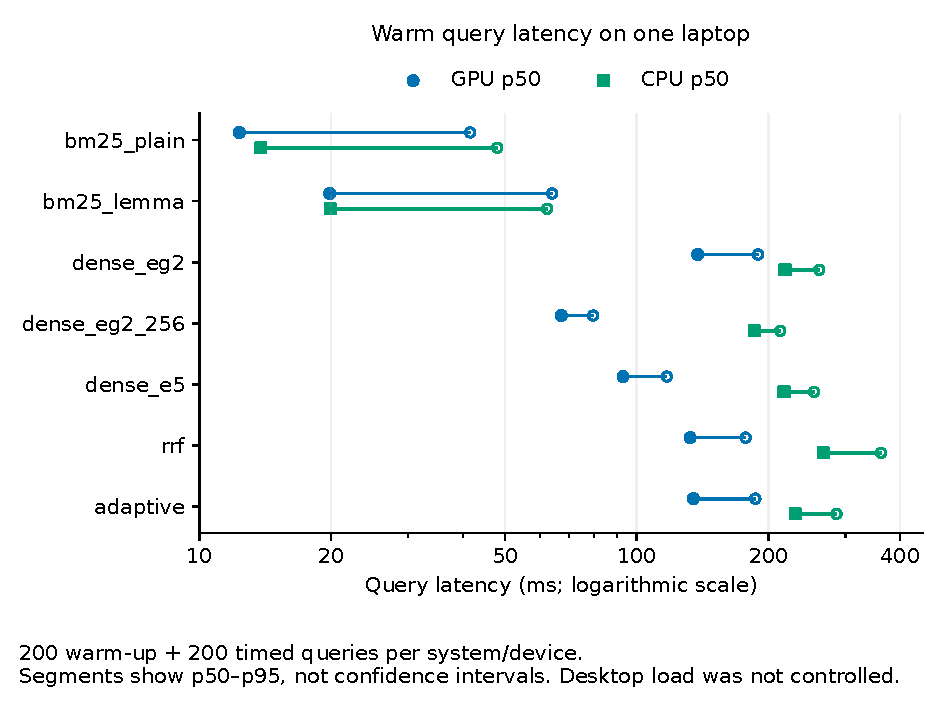
\includegraphics[width=\linewidth]{query_latency.pdf}
\caption{Затримка запитів після повного розігріву. Маркери показують p50, відкриті кінці --- p95, а не довірчі межі; горизонтальна вісь логарифмічна. Обидва прогони включають усі 200 запитів.}
\label{fig:query-latency}
\end{figure}

\begin{figure}[p]
\centering
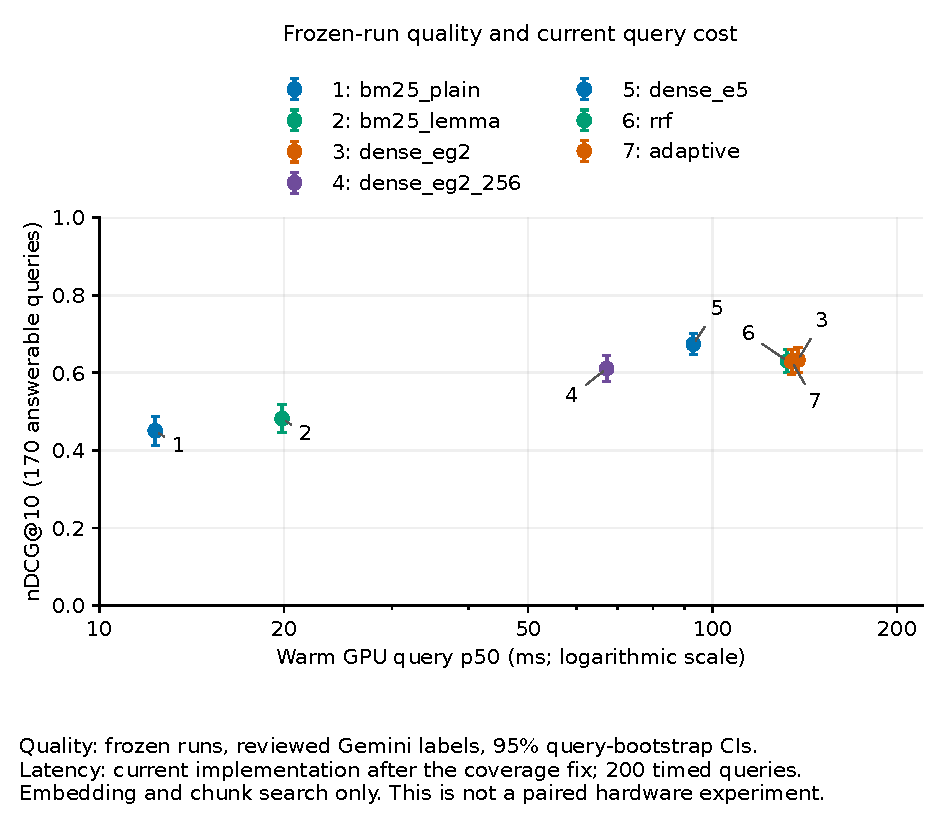
\includegraphics[width=\linewidth]{latency_quality.pdf}
\caption{Якість за початковими зафіксованими прогонами та поточна затримка запиту на GPU після розігріву. Інтервали якості використовують 170 запитів із відповіддю й переглянуті мітки Gemini; затримка --- усі 200 запитів після виправлення покриття цілих слів. Осі описують різні версії коду, як зазначено в контрольному аналізі; це не парний експеримент обладнання. Згортання до документів не входить у таймер.}
\label{fig:latency-quality}
\end{figure}
\else
\pending{Повні вимірювання затримки CPU/GPU}
\fi
\ifpaperindexing
Табл.~\ref{tab:indexing} подає GPU-вибірку з 475 файлів і CPU-вибірку з 95. Їхній склад різний; фрагменти за секунду характеризують ці прогони, а співвідношення повного часу не є парною оцінкою апаратного прискорення.
\begin{table}[p]
\centering
\caption{Індексування в порожню базу двох фіксованих вибірок різного розміру. Кількості стосуються вибраних файлів і створених фрагментів; RSS --- пік дочірнього процесу. Вибіркова БД включає службові файли; розміри повних індексів стосуються основних файлів баз.}
\label{tab:indexing}
% Generated from primary=gemini_reviewed; see ../manifest.json for source SHA-256.
% indexing a fixed sample of the corpus with the archive CLI; source efficiency.json
\begingroup\small\setlength{\tabcolsep}{4pt}\renewcommand{\arraystretch}{1.3}
\noindent\begin{tabularx}{\linewidth}{@{}l*{7}{>{\centering\arraybackslash}X}@{}}
\toprule
Пристрій & Файли & Фрагменти & Секунди & Фрагм./с & БД, МіБ & RSS, МіБ & VRAM +МіБ \\
\midrule
GPU & 475 & 5\,155 & 106.1 & 48.58 & 59.9 & 2591 & 6816 \\
CPU & 95 & 1\,187 & 1395.1 & 0.85 & 13.6 & 2979 & 0 \\
\bottomrule
\end{tabularx}\endgroup

\par\medskip
% main database files; sample disk above includes sidecars
\begingroup\small\setlength{\tabcolsep}{4pt}\renewcommand{\arraystretch}{1.3}
\noindent\begin{tabularx}{\linewidth}{@{}l*{1}{>{\centering\arraybackslash}X}@{}}
\toprule
Повний індекс & Основна БД, МіБ \\
\midrule
e5.sqlite3 & 1096.4 \\
full.sqlite3 & 1120.7 \\
noshort.sqlite3 & 1208.5 \\
plain.sqlite3 & 1094.7 \\
\bottomrule
\end{tabularx}\endgroup

\end{table}
\else
\pending{Повні вимірювання індексування CPU/GPU}
\fi

\subsection{Пошук із квантуванням}
\ifpapergguf
\begin{table}[p]
\centering
\caption{GGUF-збірки EG2 на тих самих текстових кандидатах, що й еталон bfloat16. Затримку виміряно після розігріву всіма 200 запитами. Різниці використовують переглянуті мітки Gemini та дослідницькі некориговані парні тести; неоцінені результати вважаються нерелевантними. Розміри файлів --- МіБ.}
\label{tab:gguf}
% Generated from primary=gemini_reviewed; see ../manifest.json for source SHA-256.
% dense EG2 on the 4137 text documents; labels gemini_reviewed; source efficiency.json quantization
\begingroup\small\setlength{\tabcolsep}{4pt}\renewcommand{\arraystretch}{1.3}
\noindent\begin{tabularx}{\linewidth}{@{}l*{3}{>{\centering\arraybackslash}X}@{}}
\toprule
Збірка & Файл, МіБ & Фрагм./с & Запит p50 \\
\midrule
bf16 (SentenceTransformers) & -- & -- & -- \\
f16 & 532 & 46 & 76.7 \\
Q8\_0 & 296 & 48 & 86.0 \\
Q4\_K\_M & 173 & 46 & 83.6 \\
\bottomrule
\end{tabularx}\endgroup

\par\medskip
% dense EG2 on the 4137 text documents; labels gemini_reviewed; source efficiency.json quantization
\begingroup\small\setlength{\tabcolsep}{4pt}\renewcommand{\arraystretch}{1.3}
\noindent\begin{tabularx}{\linewidth}{@{}l*{4}{>{\centering\arraybackslash}X}@{}}
\toprule
Збірка & nDCG@10 & $\Delta$ [95\% ДІ] & p & Неоцінені@10 \\
\midrule
bf16 (SentenceTransformers) & 0.631 & -- & -- & 0.003 \\
f16 & 0.631 & \shortstack{-0.001 \\ {\footnotesize[-0.005, +0.003]}} & 0.734 & 0.016 \\
Q8\_0 & 0.630 & \shortstack{-0.002 \\ {\footnotesize[-0.006, +0.003]}} & 0.504 & 0.018 \\
Q4\_K\_M & 0.613 & \shortstack{-0.018 \\ {\footnotesize[-0.030, -0.006]}} & 0.002 & 0.099 \\
\bottomrule
\end{tabularx}\endgroup

\par\medskip
% dense EG2 on the 4137 text documents; labels gemini_reviewed; source efficiency.json quantization; unjudged documents removed before ranking evaluation
\begingroup\small\setlength{\tabcolsep}{4pt}\renewcommand{\arraystretch}{1.3}
\noindent\begin{tabularx}{\linewidth}{@{}l*{3}{>{\centering\arraybackslash}X}@{}}
\toprule
Збірка & Condensed nDCG@10 & $\Delta$ [95\% ДІ] & p \\
\midrule
bf16 (SentenceTransformers) & 0.632 & -- & -- \\
f16 & 0.634 & \shortstack{+0.002 \\ {\footnotesize[-0.002, +0.006]}} & 0.297 \\
Q8\_0 & 0.633 & \shortstack{+0.000 \\ {\footnotesize[-0.004, +0.005]}} & 0.869 \\
Q4\_K\_M & 0.636 & \shortstack{+0.004 \\ {\footnotesize[-0.007, +0.015]}} & 0.454 \\
\bottomrule
\end{tabularx}\endgroup

\end{table}
\begin{figure}[p]
\centering
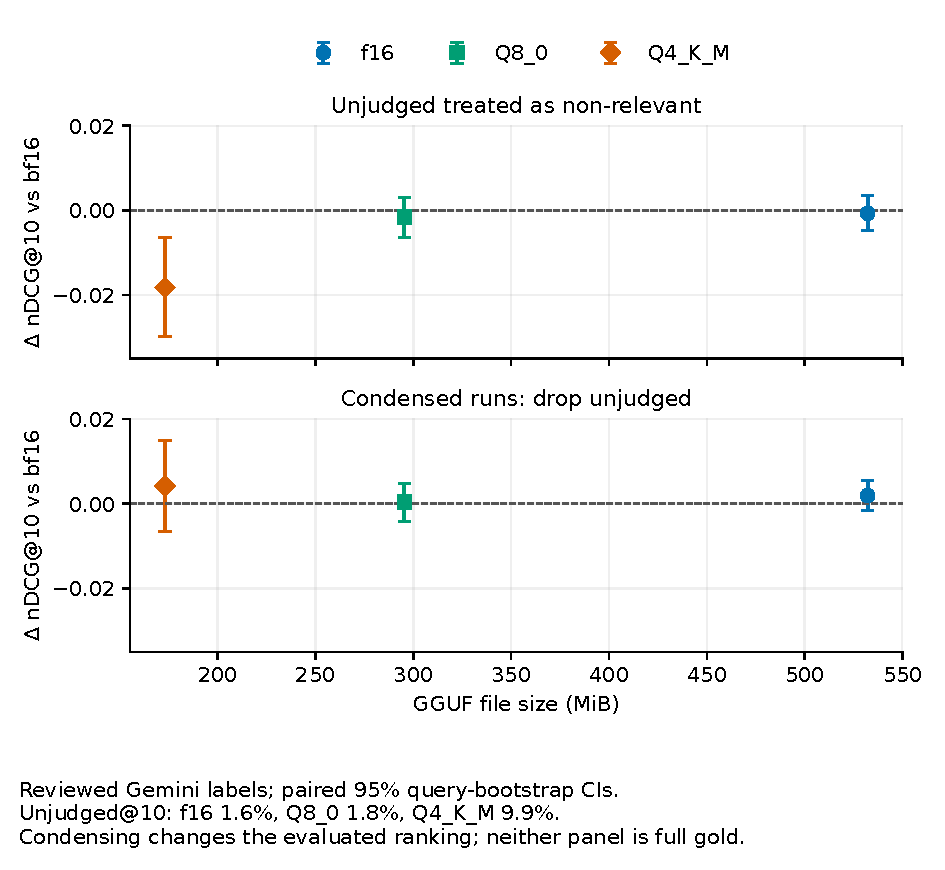
\includegraphics[width=\linewidth]{quantization_quality.pdf}
\caption{Парні різниці nDCG@10 від еталона bf16 EG2 залежно від розміру GGUF на однакових текстових кандидатах. Верхня панель вважає неоцінені документи нерелевантними, нижня --- вилучає їх. Відрізки --- 95\% бутстреп-інтервали за запитами. Залежність від охоплення оцінювання не дозволяє вважати верхню різницю Q4 ізольованим ефектом квантування.}
\label{fig:quantization-quality}
\end{figure}
Табл.~\ref{tab:gguf} показує якість пошуку, швидкість кодування та затримку запиту локального сервера. Окремий косинусний експеримент у додатку не замінює цих пошукових порівнянь. Точкові різниці f16 і Q8 від еталона bf16 малі, але інтервали, що містять нуль, не доводять еквівалентності. Для Q4 трактування неоцінених результатів як нерелевантних дає різницю $-0{,}018$ (95\% ДІ $[-0{,}030,-0{,}006]$); 9,9\% його першої десятки не оцінено проти 0,3\% для еталона. На стиснутих прогонах різниця Q4 становить $+0{,}004$ з інтервалом, що охоплює нуль. Вилучення неоцінених результатів змінює оцінюване ранжування, але не встановлює їхньої релевантності. Отже, зафіксований пул не дозволяє встановити власну втрату якості Q4. Порівняння також змінюють бекенд і числову точність, а не лише квантування.
\else
\pending{Пошуковий експеримент GGUF не завершено; косинусні оцінки наведено в додатку}
\fi

\subsection{Синтетичне масштабування}
\ifpaperann
\begin{table}[p]
\centering
\caption{Точний і наближений пошук на синтетичних колекціях зі справжніх векторів. Затримка --- p50 мілісекунд для одного запиту. Комірки HNSW містять затримку / повноту@10 відносно точного пошуку; час побудови --- секунди. Вимірюється лише пошук векторів фрагментів.}
\label{tab:ann}
% Generated from primary=gemini_reviewed; see ../manifest.json for source SHA-256.
% p50 ms per single query; HNSW cells: p50 ms / strict-ID recall@10 against exact; source ann_scaling.json
\begingroup\small\setlength{\tabcolsep}{4pt}\renewcommand{\arraystretch}{1.3}
\noindent\begin{tabularx}{\linewidth}{@{}l*{5}{>{\centering\arraybackslash}X}@{}}
\toprule
Векторів & NumPy top-k & Faiss flat & Побудова HNSW, с & HNSW ef64 & HNSW ef256 \\
\midrule
100\,000 & 6.16 & 10.65 & 9 & 0.19 / 0.914 & 0.57 / 0.984 \\
300\,000 & 17.85 & 26.52 & 33 & 0.27 / 0.940 & 0.69 / 0.990 \\
1\,000\,000 & 51.78 & 75.83 & 187 & 0.29 / 0.904 & 0.97 / 0.991 \\
2\,000\,000 & 106.63 & 139.95 & 676 & 0.39 / 0.893 & 1.28 / 0.983 \\
\bottomrule
\end{tabularx}\endgroup

\par\medskip
% Actual semantic_scored path with candidate gather, full sort, pool400; no database polling; flat exact agreement / fraction at reference kth score within1e-6; source ann_reference_audit.json
\begingroup\small\setlength{\tabcolsep}{4pt}\renewcommand{\arraystretch}{1.3}
\noindent\begin{tabularx}{\linewidth}{@{}l*{3}{>{\centering\arraybackslash}X}@{}}
\toprule
Векторів & Пошук архіву p50, мс & Збіг ID flat & Поріг оцінки flat \\
\midrule
100\,000 & 60.84 & 1.000 & 1.000 \\
300\,000 & 166.80 & 1.000 & 1.000 \\
1\,000\,000 & 497.64 & 1.000 & 1.000 \\
2\,000\,000 & 2441.83 & 1.000 & 1.000 \\
\bottomrule
\end{tabularx}\endgroup

\par\smallskip
На 2\,000\,000 векторах спостережена p50 становить 106.6 мс для оптимізованого NumPy top-k і 2441.8 мс для векторного пошуку архіву. HNSW ef256 має 1.28 мс за повноти@10 за ідентифікаторами 0.9825. Це послідовні вимірювання різних алгоритмів і розмірів видачі (10 проти 400) у робочому сеансі, а не парне прискорення обладнання чи наскрізна затримка інтерфейсу.

\end{table}
\begin{figure}[p]
\centering
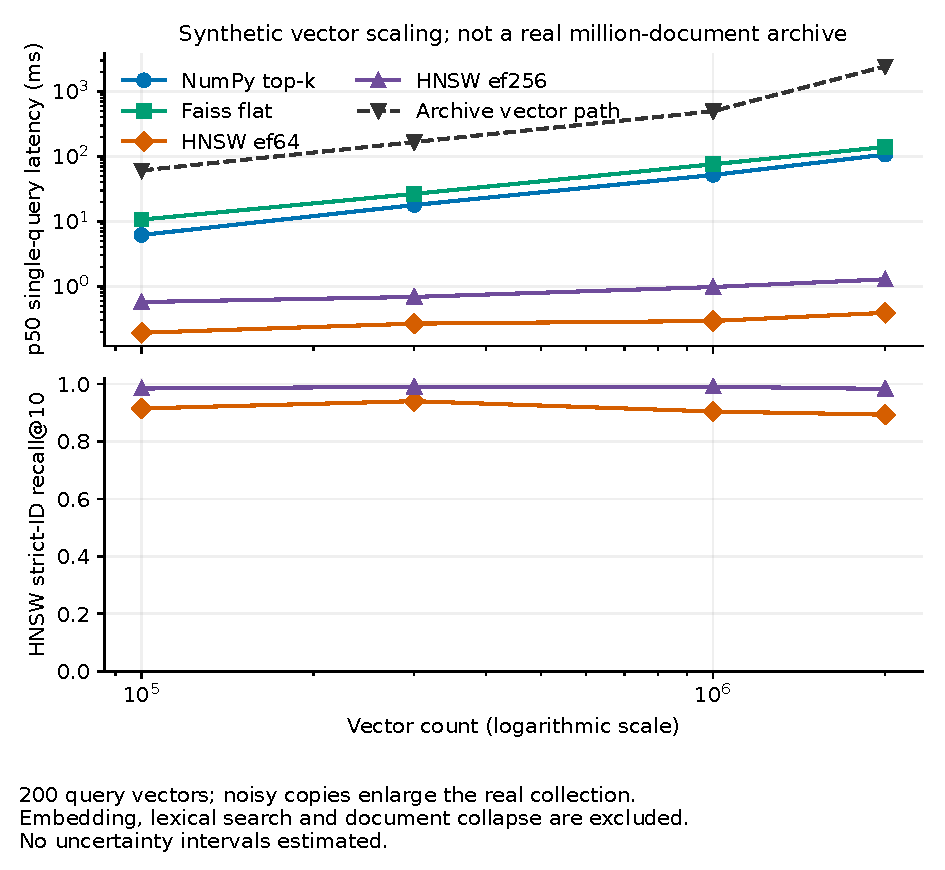
\includegraphics[width=\linewidth]{ann_scaling.pdf}
\caption{Затримка векторного пошуку й повнота HNSW на синтетично збільшених колекціях. Вісь затримки логарифмічна; інтервали невизначеності не оцінюються.}
\label{fig:ann-scaling}
\end{figure}
Табл.~\ref{tab:ann} відокремлює вартість точного векторного пошуку від наближення HNSW. Тут немає кодування запиту, лексичного пошуку та згортання документів; це не оцінка релевантності на справжньому архіві з мільйона документів.
\else
\pending{Повний експеримент масштабування exact/Faiss/HNSW}
\fi

\subsection{Додаткові типи цілей}\label{sec:results-extension}
\ifpaperextension
Окреме розширення містить 50 запитів Qwen до 20 документів, 15 таблиць і 15 файлів репозиторіїв та використовує виправлене правило покриття. Початкові мітки Gemini і Gemma~4 12B подано окремо в табл.~\ref{tab:extension}. 50 записів містять 49 різних формулювань: одне використано для двох файлів. Вони не змішуються з початковими 200 чи їхніми основними мітками релевантності. GPT використовується лише для порівняння. Відмінності між популяціями запитів не ідентифікують самопреференцію, адже також різняться авторство, тип цілі та складність.
\begin{table}[p]
\centering
\caption{nDCG@10 і 95\% бутстреп-інтервали за запитами на окремому розширенні з 50 запитів. Обидва варіанти міток --- початкові оцінки; жоден не є переглянутим основним варіантом початкового тесту.}
\label{tab:extension}
% Generated from primary=gemini_reviewed; see ../manifest.json for source SHA-256.
% nDCG@10, 95% query-bootstrap CI; separate 50-query extension; source extension.json
\begingroup\small\setlength{\tabcolsep}{4pt}\renewcommand{\arraystretch}{1.3}
\noindent\begin{tabularx}{\linewidth}{@{}l*{2}{>{\centering\arraybackslash}X}@{}}
\toprule
Система & Gemini initial & Gemma 12B initial \\
\midrule
bm25\_plain & \shortstack{0.496 \\ {\footnotesize[0.404, 0.590]}} & \shortstack{0.507 \\ {\footnotesize[0.409, 0.604]}} \\
bm25\_lemma & \shortstack{0.523 \\ {\footnotesize[0.431, 0.617]}} & \shortstack{0.540 \\ {\footnotesize[0.443, 0.639]}} \\
dense\_eg2 & \shortstack{0.759 \\ {\footnotesize[0.697, 0.817]}} & \shortstack{0.769 \\ {\footnotesize[0.701, 0.832]}} \\
dense\_e5 & \shortstack{0.721 \\ {\footnotesize[0.654, 0.785]}} & \shortstack{0.730 \\ {\footnotesize[0.666, 0.790]}} \\
rrf & \shortstack{0.684 \\ {\footnotesize[0.619, 0.749]}} & \shortstack{0.696 \\ {\footnotesize[0.623, 0.766]}} \\
adaptive & \shortstack{0.756 \\ {\footnotesize[0.694, 0.814]}} & \shortstack{0.765 \\ {\footnotesize[0.697, 0.827]}} \\
adaptive-phrase & \shortstack{0.756 \\ {\footnotesize[0.694, 0.814]}} & \shortstack{0.765 \\ {\footnotesize[0.697, 0.827]}} \\
adaptive-ident & \shortstack{0.756 \\ {\footnotesize[0.694, 0.814]}} & \shortstack{0.765 \\ {\footnotesize[0.697, 0.827]}} \\
adaptive-short & \shortstack{0.756 \\ {\footnotesize[0.694, 0.814]}} & \shortstack{0.765 \\ {\footnotesize[0.697, 0.827]}} \\
dense\_eg2\_256 & \shortstack{0.713 \\ {\footnotesize[0.639, 0.782]}} & \shortstack{0.732 \\ {\footnotesize[0.662, 0.797]}} \\
\bottomrule
\end{tabularx}\endgroup

\end{table}

За початковими мітками Gemini EG2 має 0,759, адаптивне злиття --- 0,756, E5 --- 0,721, а BM25 із лемами --- 0,523. За початковими мітками Gemma~4 12B відповідні оцінки становлять 0,769, 0,765, 0,730 і 0,540. Адаптивний метод перевершує обидва лексичні базові методи після поправки Holm за обох варіантів міток; ці тести не відокремлюють від нього ні EG2, ні E5. Зміна точкового порядку щільних енкодерів стосується цієї популяції, а не порівняння загальної складності з початковим тестом. GPT лишається найпоблажливішим і на запитах Qwen (середня оцінка 0,550 проти 0,379 у Gemini й 0,437 у Gemma), що підсилює висновок: початковий патерн GPT не ідентифікує самопреференції автора запитів.

\ifpaperextensionunique
Збереження найменшого ідентифікатора для кожного нормалізованого формулювання вилучає q249 без добору за оцінкою пошуку. Табл.~\ref{tab:extension-unique} показує цей дослідницький аналіз чутливості. Інтервали для 50 записів використовують записи як одиниці перевибірки попри спільне формулювання; окремий аналіз усуває цей дублікат, але не робить вибірку репрезентативною.
\begin{table}[p]
\centering
\caption{П'ять основних систем на підмножині унікальних формулювань розширення. Початкові мітки й бутстреп-інтервали за запитами; інші системи та парні статистики збережено в JSON результатів.}
\label{tab:extension-unique}
% Generated from primary=gemini_reviewed; see ../manifest.json for source SHA-256.
Чутливість на унікальних формулюваннях: 49 запитів.
\par\smallskip
% keep lowest qid per normalized wording; source extension.json
\begingroup\small\setlength{\tabcolsep}{4pt}\renewcommand{\arraystretch}{1.3}
\noindent\begin{tabularx}{\linewidth}{@{}l*{2}{>{\centering\arraybackslash}X}@{}}
\toprule
Система & Gemini initial & Gemma 12B initial \\
\midrule
bm25\_plain & \shortstack{0.503 \\ {\footnotesize[0.407, 0.597]}} & \shortstack{0.513 \\ {\footnotesize[0.414, 0.611]}} \\
bm25\_lemma & \shortstack{0.530 \\ {\footnotesize[0.439, 0.624]}} & \shortstack{0.546 \\ {\footnotesize[0.448, 0.646]}} \\
dense\_e5 & \shortstack{0.717 \\ {\footnotesize[0.649, 0.782]}} & \shortstack{0.724 \\ {\footnotesize[0.659, 0.786]}} \\
dense\_eg2 & \shortstack{0.757 \\ {\footnotesize[0.695, 0.813]}} & \shortstack{0.765 \\ {\footnotesize[0.698, 0.826]}} \\
adaptive & \shortstack{0.754 \\ {\footnotesize[0.692, 0.810]}} & \shortstack{0.760 \\ {\footnotesize[0.694, 0.821]}} \\
\bottomrule
\end{tabularx}\endgroup

\end{table}
\fi

\else
\pending{Окреме розширення з 50 запитів до документів, таблиць і коду та його оцінювання}
\fi

% Keep public-result floats ahead of the separate private-archive study.
\clearpage
% Приватне дослідження: лише агреговані операційні перевірки.
\section{Польове дослідження на архіві автора}\label{sec:field}

Приватне дослідження запускає реалізований адаптивний пошук на наявному архіві автора з трьома наборами запитів, написаних під час розроблення системи. Їхні назви (main, holdout7 і holdout11) --- позначення розроблення, а не свідчення незалежної вибірки чи проспективного користувацького дослідження. Набори містять відповідно 80, 86 і 214 запитів. Документи, тексти запитів, шляхи, фрагменти й індивідуальні результати не експортуються.

Виконуються три операційні перевірки. Для точного запиту успіх означає наявність очікуваної фрази у знайденому фрагменті після нормалізації пробілів і регістру; ранги й обернені ранги стосуються фрагментів. Для описового запиту успіх означає наявність очікуваного проєкту серед перших п’яти фрагментів. Для запиту без відповіді успіх означає відсутність результатів у лексичному режимі; це не перевірка утримання від відповіді векторного пошуку. Ці перевірки слабші за незалежні оцінки релевантності документів. Кожен набір і тип підсумовуються окремо з 95\% бутстреп-інтервалами за запитами; набори не об’єднуються в загальну оцінку ефективності.

\ifpaperfield
\begin{table}[!htbp]
\centering
\caption{Операційні перевірки приватного архіву: кількості, середні та 95\% бутстреп-інтервали за запитами. Для точних запитів ранги стосуються фрагментів; описові перевіряють проєкт; безвідповідні --- лексичне утримання. Експортуються лише агрегати.}
\label{tab:field}
% Generated from primary=gemini_reviewed; see ../manifest.json for source SHA-256.
Архів: 11\,394 документів, 902\,739 фрагментів.
\par\smallskip
% private archive aggregates only; exact ranks are chunk ranks; source field_aggregate.json
\begingroup\small\setlength{\tabcolsep}{4pt}\renewcommand{\arraystretch}{1.3}
\noindent\begin{tabularx}{\linewidth}{@{}l*{4}{>{\centering\arraybackslash}X}@{}}
\toprule
Набір & Тип & Запитів & Метрика & Середнє [95\% ДІ] \\
\midrule
holdout11 & exact & 192 & hit@1 & 0.672 [0.604, 0.740] \\
holdout11 & exact & 192 & hit@5 & 0.708 [0.641, 0.771] \\
holdout11 & exact & 192 & mrr@10 & 0.691 [0.627, 0.754] \\
holdout11 & absent & 10 & pass & 1.000 [1.000, 1.000] \\
holdout11 & described & 12 & hit@5 & 1.000 [1.000, 1.000] \\
holdout7 & exact & 64 & hit@1 & 0.641 [0.516, 0.750] \\
holdout7 & exact & 64 & hit@5 & 0.703 [0.594, 0.812] \\
holdout7 & exact & 64 & mrr@10 & 0.668 [0.557, 0.777] \\
holdout7 & absent & 10 & pass & 1.000 [1.000, 1.000] \\
holdout7 & described & 12 & hit@5 & 1.000 [1.000, 1.000] \\
main & exact & 66 & hit@1 & 0.697 [0.576, 0.803] \\
main & exact & 66 & hit@5 & 0.727 [0.621, 0.833] \\
main & exact & 66 & mrr@10 & 0.709 [0.598, 0.813] \\
main & absent & 8 & pass & 1.000 [1.000, 1.000] \\
main & described & 6 & hit@5 & 1.000 [1.000, 1.000] \\
\bottomrule
\end{tabularx}\endgroup

\end{table}
Табл.~\ref{tab:field} описує це середовище й ці запити розроблення. Якщо всі спостереження успішні, перцентильний бутстреп дає вироджений інтервал [1,1]; це не гарантія для популяції. Інтервали характеризують перевибірку всередині набору; вони не враховують налаштування на цьому архіві, добір запитів чи відмінності між людьми.
\else
\pending{Агрегати польового дослідження ще не отримано}
\fi

% Flush result floats before interpretation and references.
\clearpage
% Інтерпретація завершених результатів без нових вимірювань чи міток.
\section{Обговорення}\label{sec:discussion}

\paragraph{Морфологія (RQ1).}
Виправлене розширення лемами підвищує nDCG@10 BM25 на 0,031 за основними мітками з парним 95\% інтервалом від 0,013 до 0,051. Це підтримує приріст для цього набору запитів за цих оцінок. Слабші свідчення за Gemma~4 12B обмежують висновок, незалежний від судді. Попереднє погіршення до виправлення аналізатора також ілюструє залежність від реалізації: розширення неправильно вгаданою лемою може змінювати пошук у протилежний бік. Результат стосується перевіреного правила аналізатора й корпусу, а не морфології як універсально корисної операції.

\paragraph{Злиття й технічні запити (RQ2--RQ3).}
Адаптивне злиття перевищує BM25 за основною метрикою, проте виявленої переваги над EG2 чи RRF немає. E5 має найвище середнє nDCG@10, зокрема в контролі на однакових текстових кандидатах. Відсутність значущого після поправки Холма контрасту E5--adaptive не встановлює однакової ефективності. Абляція переранжування фраз чисельно тотожна повній системі на заморожених прогонах; абляції ідентифікаторів і коротких фрагментів також не підтверджують поліпшення на цій вибірці. Правило може виправляти правдоподібний збій, який трапляється тут недостатньо часто для поліпшення сукупної метрики. Загальні рекомендації щодо правила злиття тому потребували б незалежно написаних запитів і ширшого охоплення цілей.

\paragraph{Зміна охоплення цілей.}
Окреме розширення дає інший порядок: EG2 та адаптивне злиття мають вищі точкові оцінки за E5 за його початковими мітками Gemini. Між наборами також змінюються автор запитів, формати цілей і варіант оцінювання. Тому розширення не визначає, який чинник спричиняє цю відмінність, а його середні не слід вважати поліпшенням «до/після» відносно початкового тесту. Збереження аналізу всіх 50 записів поряд із детермінованою перевіркою на 49 формулюваннях утримує початкові дані й робить повтор формулювання явним.

\paragraph{Мультимодальне зіставлення (RQ4).}
Завдання «підпис--зображення» та «транскрипт--запис» перевіряють міжмодальне зіставлення двома мовами за парами з джерельних наборів. Повнота на першій позиції становить 0,857 для українських підписів і 0,889 для російських серед 1\,000 зображень. Це окремі результати від текстового пошуку з модельними оцінками. Для мовлення використання того самого транскрипту як запиту й індексованого тексту є умовою верхньої межі; навіть міжмовні транскрипти --- паралельні джерельні речення. Жодне завдання не встановлює ефективності для людського перефразування, довгого запису чи довільних фотографій. Вони підтверджують реалізований зв'язок модальностей у зазначених умовах зіставлення.

\paragraph{Квантування та охоплення оцінками (RQ5).}
Звичайне порівняння Q4 має від'ємну точкову різницю, тоді як конденсоване оцінювання не показує такого самого погіршення; 9,9\% результатів Q4 у першій десятці не оцінено. Тому звичайна метрика за замороженим пулом не ідентифікує внутрішньої втрати релевантності Q4. Водночас малі відмінності f16/Q8 та інтервали, що охоплюють нуль, не встановлюють еквівалентності. Бекенд і точність змінюються разом, а для 21 рядка PDF-сторінок змінюється ще й вхідна модальність. Якість, розмір файлів і витрати кодування слід читати разом із цими умовами охоплення та реалізації, а не як ізольований причинний ефект квантування.

\paragraph{Витрати фактичного пошукового шляху.}
На двох мільйонах синтетичних векторів медіана фактичного шляху ранжування архіву становить близько 2\,442~мс, а оптимізованого еталона NumPy для першої десятки --- близько 107~мс. Шляхи виконують різну роботу: метод архіву збирає кандидатів, повністю сортує оцінки й формує 400 кортежів. Різниця виявляє роботу реалізації, яку приховав би опис лише множення матриці на вектор. HNSW із глибиною пошуку 256 витрачає близько 1,28~мс і має recall@10 за точним збігом ідентифікаторів 0,9825 на цій синтетичній колекції. Послідовні вимірювання у звичайній робочій сесії не є оцінкою наскрізного чи парного прискорення; повнота може не переноситися на реальний архів такого розміру. Це обґрунтовує приблизну індексацію та відбір кандидатів як подальші напрями інженерної роботи.

\paragraph{Оцінювання та практична інтерпретація.}
Узгодженість суддів, перевірки цільових документів і навмисно безвідповідні запити характеризують поведінку оцінювання, проте не встановлюють відповідності людським судженням. Перегляд Gemini зберігає залежність від початкових суддів і видимих оцінок, тому точкові результати супроводжуються аналізом чутливості до міток. Незалежне людське дослідження та запити людей, які шукають власні документи, залишаються майбутньою перевіркою й не подаються тут як виконані. Перевірки приватного архіву показують задоволення операційних очікувань автора в цьому середовищі, проте повторне використання під час розроблення не дозволяє заявляти ефективність для користувачів. Разом ці свідчення дають доступний для перевірки опис якості й витрат на одному побудованому бенчмарку та в одному робочому архіві; найсильніші порівняння залежать від міток, вибірок і меж вимірювання.

% Обмеження і загрози валідності.
\section{Обмеження і загрози валідності}\label{sec:limitations}

\subsection{Корпус і запити}
\uapar{} імітує особистий архів відкритими матеріалами: статті Вікіпедії представляють нотатки, а їхні перетворені версії --- офісні документи. Тому текст однорідніший і краще відредагований за справжні нотатки, а приватних матеріалів у ньому немає. 200 запитів написала одна модель за правилами, а не люди, що шукали власні документи; усі цілі запитів із відповіддю --- нотатки. Окреме розширення з 50 запитів охоплює документи, таблиці й файли репозиторіїв (розділ~\ref{sec:results-extension}), але також написане моделлю. Воно містить 49 різних формулювань, тому 50 записів не цілком незалежні; окремо подано детермінований аналіз чутливості на унікальних формулюваннях. Запити без відповіді за побудовою не мають лексичних збігів, що наперед визначає результат лексичних систем на них. Теми відповідають інтересам автора; інший архів може сприяти іншим системам.

\subsection{Оцінки релевантності від мовних моделей}
Текстову релевантність оцінюють мовні моделі, а не незалежна група людей. Узгодженість, перевірки цільових документів і навмисно безвідповідних запитів дають діагностичні свідчення, проте не утворюють повного еталона. Gemini та Gemma можуть мати спільні помилки через спільного постачальника. Повторний перегляд Gemini не усуває цю залежність; крім того, під час нього видно початкові оцінки. Тому початкові мітки зберігаються, а метрики й порядок систем порівнюються за різними суддями та до і після перегляду. Основного суддю обрано після аналізу його діагностики --- це методичне рішення, ухвалене після отримання оцінок. Ця версія свідомо не містить людського аудиту релевантності. Тому висновки щодо текстового пошуку залежать від модельних суджень; незалежна людська перевірка є майбутньою роботою.

\subsection{Охоплення запитів і кандидатів}
Корпус неоднорідний, але всі задані цілі запитів із відповіддю в початковому наборі з 200 запитів --- нотатки. Окреме розширення додає малу вибірку документів, таблиць і файлів репозиторіїв. Жоден набір не встановлює загальної якості для довільних форматів цілей, зображень чи записів. E5 шукає в меншому текстовому наборі документів, а індекси EG2 включають медіа. Контроль на однакових кандидатах (табл.~\ref{tab:encoder-control}) змінює nDCG@10 EG2 на $-0{,}0015$ --- малу точкову величину в цьому контролі. Це не усуває всієї невизначеності щодо охоплення: контрольні прогони не формували пул, а 0,29\% документів їхньої першої десятки не оцінено.

Повністю оцінено лише об'єднання перших десяти результатів усіх систем. Поза пулом можуть бути релевантні документи. Повнота на глибині 100 визначається відносно відомих релевантних документів пулу; зарахування неоцінених документів до нерелевантних може сприяти системам, які формували пул, і не вимірює повноту за всім корпусом. Відсутність статистично значущої різниці не доводить еквівалентності.

\subsection{Польове дослідження одного автора}
Польове дослідження (розділ~\ref{sec:field}) використовує архів однієї людини та набори запитів, які автор писав під час розроблення системи, зокрема для її перевірки. Це не випадкова вибірка реальних інформаційних потреб, а систему налаштовували на тому самому архіві. Результати характеризують поведінку в цьому середовищі, а не узагальнювану ефективність.

\subsection{Вимірювання}
Усі вимірювання витрат стосуються одного ноутбука у звичайному сеансі з іншими програмами; навантаження перед кожним кроком записується, але не контролюється. Таймер запиту охоплює кодування й пошук фрагментів, але не згортання до документів, визначення шляхів і відображення інтерфейсу. Лічильники ресурсів процесу охоплюють увесь виміряний прохід, включно зі згортанням, тому їхня область вимірювання відрізняється від таймера запиту. Індексування на CPU виміряно на п'ятій частині вибірки GPU. Експеримент масштабування використовує синтетичні вектори, утворені зі справжніх; повнота HNSW на них може відрізнятися від повноти на реальній колекції такого розміру.

\subsection{Валідність вимірюваних понять}
Судді бачать назву й перші 1\,200 символів документа, а не весь документ. Тому релевантність, що проявляється лише далі, може бути недооцінена; однаковий фрагмент показується для всіх систем, проте це сприяє документам із релевантністю на початку. Оцінки 0/1/2 стискають судження, які люди можуть робити інакше: модельне «частково релевантний» не дорівнює людському. Основна метрика nDCG@10 за мітками пулу винагороджує високе ранжування оцінених релевантних документів; вона не вимірює, чи людина швидше знаходить те, що пам'ятає.

\subsection{Завдання зіставлення джерельних пар}
Завдання із зображеннями й мовленням визначають пов'язаний джерельний об'єкт або речення. Ці пари не дають вичерпних оцінок кожного семантично спорідненого кандидата. Підписи й паралельні транскрипти також відрізняються від незалежно перефразованих запитів до архіву. Для поданих точкових оцінок довірчі інтервали не обчислювалися.

% Ідентифікатори випуску очікують рішення автора; DOI прикладів не використовуються повторно.
\section{Доступність даних і коду}\label{sec:availability}

\paragraph{Дослідницькі матеріали.}
Публічний випуск для авторського огляду містить виконуваний код, збережені результати JSON, джерела рукопису, згенеровані таблиці й рисунки та обидва PDF за адресою \url{https://github.com/cyberdid/archive-index-public}, тег \code{paper-author-review-2026-10-23-r2}. DOI програмних матеріалів і препринту ще не присвоєно. Маніфест таблиць пов’язує числові матеріали з хешами джерел. Публічний пакет дає змогу перебудувати таблиці й PDF зі збережених результатів. Повний заморожений корпус, входи запитів, прогонів та оцінювання і їх 14-етапне відтворення збережені в окремому дослідницькому архіві; цей випуск їх не поширює, доки перевірка сторонньої атрибуції та сфери прав не завершена. Точне наскрізне статистичне відтворення тому потребує цих окремо збережених входів. Скрипти побудови корпусу й оцінювання оприлюднені.

\paragraph{Відтворення.}
Ізольований засіб \path{paper/run_all.sh} розрізняє складання зі збережених результатів і повне статистичне відтворення заморожених входів. Виконаний повний прохід має 14 етапів і відтворює десять звітів, канонічні qrels та записані хеші входів ANN. Фізичні вимірювання витрат, мультимодальних завдань, ANN і приватного архіву в цьому проході імпортуються, а не виконуються повторно. Зафіксовані 315 тестів реалізації, зокрема інтеграційна перевірка локально кешованої справжньої моделі, окремо характеризують поведінку коду. Разом із ним надаються описи спостереженого середовища та вимоги, зафіксовані хешами; нове повне встановлення CUDA не заявляється. Перебудова таблиць чи PDF сама по собі не повторює модельного оцінювання або фізичних вимірювань.

\paragraph{Політика джерел та атрибуція.}
Для кожного файла маніфест містить адресу джерела, зібрану ліцензійну мітку та SHA-256. Нотатки й зверстані документи походять з української та російської Вікіпедії (CC~BY-SA~4.0); 150 вибраних таблиць data.gov.ua мають мітки CC~BY. Для зображень Crossmodal-3600 збережено атрибуцію кожного зображення під CC~BY~2.0, підписи мають CC~BY~4.0; записи й транскрипти FLEURS --- CC~BY~4.0. Відбір репозиторіїв допускав мітки API MIT або Apache-2.0; зібрані репозиторії коду позначені MIT у маніфесті. Мітка репозиторію не визначає ліцензію кожного вкладеного матеріалу. Чинними залишаються сторонні повідомлення: інвентар атрибуції фіксує, зокрема, повідомлення SIL~OFL для шрифту Rubik, прив'язане до ревізії доповнення відсутньої ліцензії та питання сфери дії умов застосунку. Початкові повідомлення, файли атрибуції та аудит у \path{paper/corpus/LICENSES.md} збережено. Остаточна перевірка прав на поширення сторонніх матеріалів залишається невиконаною.

\paragraph{Ліцензування.}
Власний виконуваний код поширюється за Apache License~2.0. Текст статті, оригінальні рисунки й експериментальні записи --- за Creative Commons Attribution~4.0 International (\url{https://creativecommons.org/licenses/by/4.0/}) у межах прав автора. Посібник із ліцензування розмежовує ці матеріали та сторонні файли корпусу й залежності, для яких збережено власні умови.

\paragraph{Приватні дані та перевірка випуску.}
З архіву автора експортуються лише агреговані операційні перевірки; документи, тексти запитів, шляхи, фрагменти й індекс виключено. Перевірка випуску охоплює назви файлів, байти відомих маркерів, декодований JSON, витягнутий текст і метадані PDF та підтримуваний стиснений вміст. Чотири перевірені збіги з публічними словами/назвами потребують явних відомостей про джерело й точного хешу файла; для повних приватних запитів і домашніх шляхів винятків немає. Це не універсальна гарантія приватності й не OCR-перевірка зображень. Наявна приватна історія Git непридатна як публічний випуск; публікація потребує окремо перевіреного експорту.

\paragraph{Моделі та програмне забезпечення.}
Записи експериментів ідентифікують EmbeddingGemma~2 (\code{google/embeddinggemma-2}, ревізія \code{914f7f8}), multilingual-E5-large (\code{intfloat/multilingual-e5-large}), збірки llama.cpp/GGUF та кожну модель-суддю. Відбитки пакетів, моделей і команд залишаються прив'язаними до відповідних прогонів. Ваги моделей не входять до дослідницького експорту.

\paragraph{Участь ШІ.}
Модельне написання запитів та оцінювання релевантності описано в розділі~\ref{sec:uapar} й окремому аналізі розширення; оцінки GPT залишаються лише порівняльними. Claude і Codex допомагали реалізації та підготовці рукопису; робочий процес Scientific Agent Skills~\citep{kassis2026skills} використовувався для перевірок джерел і тверджень. Автор відповідає за план дослідження, інтерпретації, посилання та остаточні декларації. Жодна система ШІ не є автором. Ця версія не містить людського аудиту текстової релевантності; мультимодальні пари з джерельних наборів і перевірки реалізації його не замінюють.

% Висновки залежать від дослідженого архіву, міток і меж вимірювання.
\section{Висновки}\label{sec:conclusion}

Дослідження робить пошукові рішення archive-index доступними для перевірки завдяки побудованій багатомовній колекції, замороженим запитам і прогонам, збереженим модельним оцінкам та генерованим звітам. За основними переглянутими мітками Gemini на 170 запитах із відповіддю середнє nDCG@10 становить 0,674 для E5, 0,633 для EG2, 0,629 для адаптивного злиття, 0,482 для BM25 із лемами та 0,450 для звичайного BM25. Адаптивне злиття перевищує BM25 після поправки, проте ці дані не встановлюють переваги над EG2 чи RRF. Свідчення користі морфології залежать від судді, а окреме розширення показує зміну точкового порядку енкодерів між наборами.

Ширший результат --- виміряний опис компромісів реалізації й оцінювання. Пошук із квантованими збірками залежить від охоплення оцінками та відмінностей входів/бекендів; синтетичне масштабування відділяє оптимізований відбір векторів від фактичного шляху ранжування архіву; мультимодальні завдання та перевірки приватного архіву відповідають на вужчі питання, ніж ефективність текстового пошуку для людини. Результати стосуються побудованого бенчмарку з модельними оцінками релевантності. Незалежні людські оцінки, незалежно сформульовані інформаційні потреби й перевірка на різних архівах залишаються майбутньою валідацією перед загальними твердженнями про пошук в особистих архівах.


\bibliographystyle{plainnat}
\bibliography{../refs}

\appendix
\clearpage
\section{Детальні результати вимірювань}
Наведені фрагменти генеруються з тих самих файлів, що й основні таблиці. Контрольні суми джерел та поточний основний варіант релевантності записано в \path{generated/manifest.json}.
\subsection{Стан оцінювання й межі висновків}
% Generated from primary=gemini_reviewed; see ../manifest.json for source SHA-256.
\begingroup\raggedright
Оцінювання: Gemini: перегляд тією самою моделлю. Метрики: 170 запитів із відповіддю; без відповіді: 30.
\par
R@100 відносно пулу; повної еталонної розмітки немає. Gemini та Gemma12 мають спільного розробника. Перегляд Gemini виконується тією самою моделлю. GPT не включено до основних таблиць і рисунків.
\par
gemini: 5572 оцінених пар.
\par
gemma4-12b: 5572 оцінених пар.
\par
Початкові розбіжності: 1091/5572; лінійно зважена каппа Коена: 0.652.
\par
Цільові документи: всього=170, у пулі=134, поза пулом=36. Знаменник оцінок цільових документів=134.
\par
Зібрані файли та індексовані документи є різними сукупностями.
\par
Текстовий індекс E5 та повний індекс не мають однакового набору документів.
\par
Типи цільових документів: нотатки=170. Якість для решти типів не встановлено.
\par\endgroup

\subsection{Зібрані й проіндексовані дані}
% Generated from primary=gemini_reviewed; see ../manifest.json for source SHA-256.
% Collected files and indexed documents are different populations; E5 text-only and full indexes do not share the same document universe.
\begingroup\small\setlength{\tabcolsep}{4pt}\renewcommand{\arraystretch}{1.3}
\noindent\begin{tabularx}{\linewidth}{@{}l*{1}{>{\centering\arraybackslash}X}@{}}
\toprule
Сукупність & Кількість \\
\midrule
Зібрані файли & 7070 \\
Запити (усі) & 200 \\
Документи індексу e5 & 4137 \\
Документи індексу full & 6054 \\
Документи індексу noshort & 6054 \\
Документи індексу plain & 6054 \\
e5: усі фрагменти & 94970 \\
e5: вектори & 84767 \\
e5: вектори текстових колекцій & 84767 \\
full: усі фрагменти & 96908 \\
full: вектори & 86726 \\
full: вектори текстових колекцій & 84788 \\
noshort: усі фрагменти & 97652 \\
noshort: вектори & 87441 \\
noshort: вектори текстових колекцій & 85503 \\
plain: усі фрагменти & 96908 \\
plain: вектори & 86726 \\
plain: вектори текстових колекцій & 84788 \\
\bottomrule
\end{tabularx}\endgroup

\clearpage
\subsection{Абляції}
% Generated from primary=gemini_reviewed; see ../manifest.json for source SHA-256.
% Means with 95% bootstrap CI; n=170. R@100 is pool-relative under incomplete judgments. Significance: paired comparison against adaptive only, \(p_{\mathrm{Holm}}<0.05\).
\begingroup\small\setlength{\tabcolsep}{4pt}\renewcommand{\arraystretch}{1.3}
\noindent\begin{tabularx}{\linewidth}{@{}l*{3}{>{\centering\arraybackslash}X}@{}}
\toprule
Система & nDCG@10 & R@100\textsuperscript{pool} & RR@10 \\
\midrule
adaptive & \shortstack{0.629 \\ {\footnotesize[0.596, 0.660]}} & \shortstack{0.908 \\ {\footnotesize[0.887, 0.928]}} & \shortstack{0.866 \\ {\footnotesize[0.826, 0.905]}} \\
adaptive-phrase & \shortstack{0.629 \\ {\footnotesize[0.596, 0.660]}} & \shortstack{0.908 \\ {\footnotesize[0.887, 0.928]}} & \shortstack{0.866 \\ {\footnotesize[0.826, 0.905]}} \\
adaptive-ident & \shortstack{0.629 \\ {\footnotesize[0.597, 0.661]}} & \shortstack{0.912 \\ {\footnotesize[0.892, 0.931]}} & \shortstack{0.866 \\ {\footnotesize[0.826, 0.905]}} \\
adaptive-short & \shortstack{0.629 \\ {\footnotesize[0.597, 0.660]}} & \shortstack{0.908 \\ {\footnotesize[0.887, 0.928]}} & \shortstack{0.866 \\ {\footnotesize[0.826, 0.905]}} \\
dense\_eg2\_256 & \shortstack{0.611 \\ {\footnotesize[0.577, 0.643]}} & \shortstack{0.888\textsuperscript{\textdagger} \\ {\footnotesize[0.863, 0.911]}} & \shortstack{0.873 \\ {\footnotesize[0.830, 0.913]}} \\
\bottomrule
\end{tabularx}\endgroup

\par\medskip
% Means with 95% bootstrap CI; n=170. R@100 is pool-relative under incomplete judgments. Significance: paired comparison against adaptive only, \(p_{\mathrm{Holm}}<0.05\).
\begingroup\small\setlength{\tabcolsep}{4pt}\renewcommand{\arraystretch}{1.3}
\noindent\begin{tabularx}{\linewidth}{@{}l*{2}{>{\centering\arraybackslash}X}@{}}
\toprule
Система & Success@1 & Success@5 \\
\midrule
adaptive & \shortstack{0.782 \\ {\footnotesize[0.718, 0.841]}} & \shortstack{0.971 \\ {\footnotesize[0.941, 0.994]}} \\
adaptive-phrase & \shortstack{0.782 \\ {\footnotesize[0.718, 0.841]}} & \shortstack{0.971 \\ {\footnotesize[0.941, 0.994]}} \\
adaptive-ident & \shortstack{0.782 \\ {\footnotesize[0.718, 0.841]}} & \shortstack{0.971 \\ {\footnotesize[0.941, 0.994]}} \\
adaptive-short & \shortstack{0.782 \\ {\footnotesize[0.718, 0.841]}} & \shortstack{0.971 \\ {\footnotesize[0.941, 0.994]}} \\
dense\_eg2\_256 & \shortstack{0.818 \\ {\footnotesize[0.759, 0.871]}} & \shortstack{0.953 \\ {\footnotesize[0.918, 0.982]}} \\
\bottomrule
\end{tabularx}\endgroup

\par\smallskip
{\footnotesize \textdagger: p\textsubscript{Holm}<0.05, adaptive; R@100: відносно пулу.}

\clearpage
\subsection{Категорії запитів}
% Generated from primary=gemini_reviewed; see ../manifest.json for source SHA-256.
% nDCG@10; source subgroup 95% bootstrap CIs; primary=gemini_reviewed.
\begingroup\small\setlength{\tabcolsep}{4pt}\renewcommand{\arraystretch}{1.3}
\noindent\begin{tabularx}{\linewidth}{@{}l*{2}{>{\centering\arraybackslash}X}@{}}
\toprule
Система & Відомий об’єкт & Тематичні \\
\midrule
bm25\_plain & \shortstack{0.475 \\ {\footnotesize[0.397, 0.552]}} & \shortstack{0.351 \\ {\footnotesize[0.296, 0.407]}} \\
bm25\_lemma & \shortstack{0.524 \\ {\footnotesize[0.451, 0.594]}} & \shortstack{0.388 \\ {\footnotesize[0.338, 0.438]}} \\
dense\_eg2 & \shortstack{0.617 \\ {\footnotesize[0.549, 0.683]}} & \shortstack{0.568 \\ {\footnotesize[0.513, 0.619]}} \\
dense\_e5 & \shortstack{0.729 \\ {\footnotesize[0.682, 0.773]}} & \shortstack{0.662 \\ {\footnotesize[0.617, 0.706]}} \\
rrf & \shortstack{0.639 \\ {\footnotesize[0.584, 0.690]}} & \shortstack{0.564 \\ {\footnotesize[0.517, 0.609]}} \\
adaptive & \shortstack{0.612 \\ {\footnotesize[0.542, 0.680]}} & \shortstack{0.568 \\ {\footnotesize[0.513, 0.619]}} \\
adaptive-phrase & \shortstack{0.612 \\ {\footnotesize[0.542, 0.680]}} & \shortstack{0.568 \\ {\footnotesize[0.513, 0.619]}} \\
adaptive-ident & \shortstack{0.612 \\ {\footnotesize[0.542, 0.680]}} & \shortstack{0.568 \\ {\footnotesize[0.513, 0.619]}} \\
adaptive-short & \shortstack{0.612 \\ {\footnotesize[0.543, 0.681]}} & \shortstack{0.569 \\ {\footnotesize[0.514, 0.620]}} \\
dense\_eg2\_256 & \shortstack{0.596 \\ {\footnotesize[0.527, 0.664]}} & \shortstack{0.539 \\ {\footnotesize[0.479, 0.598]}} \\
\bottomrule
\end{tabularx}\endgroup

\par\medskip
% nDCG@10; source subgroup 95% bootstrap CIs; primary=gemini_reviewed.
\begingroup\small\setlength{\tabcolsep}{4pt}\renewcommand{\arraystretch}{1.3}
\noindent\begin{tabularx}{\linewidth}{@{}l*{2}{>{\centering\arraybackslash}X}@{}}
\toprule
Система & Технічні & Міжмовні \\
\midrule
bm25\_plain & \shortstack{0.649 \\ {\footnotesize[0.597, 0.702]}} & \shortstack{0.351 \\ {\footnotesize[0.273, 0.427]}} \\
bm25\_lemma & \shortstack{0.651 \\ {\footnotesize[0.595, 0.706]}} & \shortstack{0.388 \\ {\footnotesize[0.302, 0.472]}} \\
dense\_eg2 & \shortstack{0.785 \\ {\footnotesize[0.746, 0.823]}} & \shortstack{0.582 \\ {\footnotesize[0.512, 0.650]}} \\
dense\_e5 & \shortstack{0.663 \\ {\footnotesize[0.606, 0.716]}} & \shortstack{0.639 \\ {\footnotesize[0.563, 0.709]}} \\
rrf & \shortstack{0.779 \\ {\footnotesize[0.734, 0.824]}} & \shortstack{0.554 \\ {\footnotesize[0.486, 0.619]}} \\
adaptive & \shortstack{0.772 \\ {\footnotesize[0.732, 0.810]}} & \shortstack{0.582 \\ {\footnotesize[0.512, 0.650]}} \\
adaptive-phrase & \shortstack{0.772 \\ {\footnotesize[0.732, 0.810]}} & \shortstack{0.582 \\ {\footnotesize[0.512, 0.650]}} \\
adaptive-ident & \shortstack{0.775 \\ {\footnotesize[0.736, 0.813]}} & \shortstack{0.582 \\ {\footnotesize[0.512, 0.650]}} \\
adaptive-short & \shortstack{0.772 \\ {\footnotesize[0.732, 0.810]}} & \shortstack{0.580 \\ {\footnotesize[0.510, 0.648]}} \\
dense\_eg2\_256 & \shortstack{0.757 \\ {\footnotesize[0.716, 0.796]}} & \shortstack{0.579 \\ {\footnotesize[0.508, 0.648]}} \\
\bottomrule
\end{tabularx}\endgroup

\clearpage
\subsection{Мови запитів}
% Generated from primary=gemini_reviewed; see ../manifest.json for source SHA-256.
% nDCG@10; source subgroup 95% bootstrap CIs; primary=gemini_reviewed.
\begingroup\small\setlength{\tabcolsep}{4pt}\renewcommand{\arraystretch}{1.3}
\noindent\begin{tabularx}{\linewidth}{@{}l*{2}{>{\centering\arraybackslash}X}@{}}
\toprule
Система & Російська & Українська \\
\midrule
bm25\_plain & \shortstack{0.421 \\ {\footnotesize[0.368, 0.474]}} & \shortstack{0.466 \\ {\footnotesize[0.417, 0.515]}} \\
bm25\_lemma & \shortstack{0.480 \\ {\footnotesize[0.428, 0.531]}} & \shortstack{0.483 \\ {\footnotesize[0.436, 0.530]}} \\
dense\_eg2 & \shortstack{0.633 \\ {\footnotesize[0.582, 0.683]}} & \shortstack{0.633 \\ {\footnotesize[0.592, 0.672]}} \\
dense\_e5 & \shortstack{0.664 \\ {\footnotesize[0.612, 0.712]}} & \shortstack{0.679 \\ {\footnotesize[0.647, 0.710]}} \\
rrf & \shortstack{0.624 \\ {\footnotesize[0.579, 0.668]}} & \shortstack{0.634 \\ {\footnotesize[0.596, 0.671]}} \\
adaptive & \shortstack{0.623 \\ {\footnotesize[0.572, 0.674]}} & \shortstack{0.631 \\ {\footnotesize[0.591, 0.670]}} \\
adaptive-phrase & \shortstack{0.623 \\ {\footnotesize[0.572, 0.674]}} & \shortstack{0.631 \\ {\footnotesize[0.591, 0.670]}} \\
adaptive-ident & \shortstack{0.625 \\ {\footnotesize[0.574, 0.676]}} & \shortstack{0.631 \\ {\footnotesize[0.591, 0.670]}} \\
adaptive-short & \shortstack{0.623 \\ {\footnotesize[0.572, 0.674]}} & \shortstack{0.632 \\ {\footnotesize[0.591, 0.670]}} \\
dense\_eg2\_256 & \shortstack{0.637 \\ {\footnotesize[0.584, 0.689]}} & \shortstack{0.597 \\ {\footnotesize[0.553, 0.640]}} \\
\bottomrule
\end{tabularx}\endgroup

\subsection{Еталон квантування}
Еталон вимірює косинусну узгодженість векторів на 20 текстах і час CPU на текст. Він не вимірює втрату якості пошуку та не встановлює затримку в експлуатації.
\par\medskip
% Generated from primary=gemini_reviewed; see ../manifest.json for source SHA-256.
% External quantization reference: embedding cosine agreement, not retrieval quality. Point estimates; no CI available. Prompt counts: f16=20, Q8_0=20, Q4_K_M=20
\begingroup\small\setlength{\tabcolsep}{4pt}\renewcommand{\arraystretch}{1.3}
\noindent\begin{tabularx}{\linewidth}{@{}l*{4}{>{\centering\arraybackslash}X}@{}}
\toprule
GGUF & Середній косинус & Найменший косинус & МБ & CPU с/текст \\
\midrule
f16 & 0.99995 & 0.99994 & 532.1 & 0.061 \\
Q8\_0 & 0.99972 & 0.99892 & 295.5 & 0.069 \\
Q4\_K\_M & 0.99043 & 0.98503 & 173.3 & 0.053 \\
\bottomrule
\end{tabularx}\endgroup

\par

\clearpage
% Preserved provenance, moved from the introduction.
\section{Виправлення реалізації та зміни протоколу}\label{sec:intro-history}
Під час розроблення змінювалися реалізація й протокол оцінювання. Наведений запис розрізняє виправлення до заморожених прогонів і пізніший контроль покриття.
\begin{enumerate}
\item \emph{Леми, вигадані аналізатором іншої мови.} Слова без суто українських літер проходили обидва аналізатори, і той, що не знав слова, вигадував лему (\emph{навчанню}$\to$\emph{навчаннить}). У першій діагностиці за цільовими документами лематизований BM25 знаходив ціль у першій десятці для 45,3\% запитів із відповіддю проти 49,4\% без лем; після виправлення --- для 50,0\%. Усі подані прогони використовують виправлений аналізатор.
\item \emph{Перебудовані терми відрізнялися від проіндексованих} для зображень і звуку, тож абляційний індекс, зроблений перебудовою термів, не був тотожний побудованому з нуля. Виправлено до прогонів, використаних тут.
\item \emph{Відносний шлях до корпусу} записав документи двічі в абляційному індексі. Виявлено й виправлено до оцінювання будь-якого прогону.
\item \emph{Фрагменти для суддів лише із заголовків.} У першому аркуші оцінювання 393 з 5\,572 пар показували судді менше 200 символів, здебільшого назву і рядок джерела. Фрагмент змінено на початок документа ще до використання будь-яких оцінок.
\item \emph{Авторство запитів.} Перший файл запитів називав автором Claude, хоча запити написала GPT-6-Luna; це виправлено до оцінювання, а оцінки GPT потім не включено до міток.
\item \emph{Покриття за підрядками в адаптивному правилі.} Перевірка точної фрази рахувала підрядки (\code{36} всередині \code{1366}). Ваду знайдено після заморожування прогонів; подано заморожені прогони, а поруч --- прогони з виправленим правилом (воно змінює першу десятку для одного запиту з 200).
\item \emph{Зміна протоколу релевантності.} План називав основним суддею Claude. Після діагностики суддів і до обчислення поданого сукупного порівняння систем автор обрав основним суддею Gemini. Пізніший частковий прохід Claude відкладено за рішенням автора й виключено з усіх наведених аналізів. Це рішення ухвалено постфактум, і так його й подано.
\end{enumerate}

\end{document}
